\chapter{Implementation}
\label{chap:implementation}
This chapter consists of implementation details for all relevant redirected walking components as well as an overview of the game design for the developed ''Ensemble Retriever'' game. The game design overview is used to provide examples and documentation on how distractors have been fully integrated into the experience itself. 

\section{Open Source Repository - GitHub}
The source code and project assets for Ensemble Retriever can be found in a publicly available GitHub Repository~\cite{projectRepository}. It should be noted that the game itself is an extension of a small prototype that was previously developed for the IMT4894 - Advanced Project Work course. This prototype consisted of no redirected walking elements and featured a battle in VR against an angry contrabass enemy. The majority of the source code has needed to be rewritten or refactored to facilitate a more generic architecture that supports the larger scope of the current game.  

\subsection{Licensing and Attribution}
Ensemble Retriever makes liberal use of royalty-free assets as a means to fasten then development time of the game. As such, it is also necessary to properly provide attribution to these assets. In general, each royalty free asset in the repository includes a corresponding license file which details the specific license that applies to it. The following list gives an overview of the royalty-free assets that were used for the project:
\begin{itemize}
    \item Most Particle effects.
    \item Fonts.
    \item Some 3D Models like hats/crowns, conducting baton, objective arrow and the cave walls in the ''Hall of The Mountain King''.
    \item Skybox.
    \item Music.
    \item Sound effects.
\end{itemize}
Those with interest in reusing or extending the project need to follow the licensing terms that apply for all of these assets. There are also specific 3D models that were reused from a previous project with permission from their creator, Yijie Zhou. These can be found in the \emph{''Assets/Meshes/BlenderAssets/''} folder of the repository and include:
\begin{itemize}
    \item All instrument 3D models.
    \item The virtual environment, excluding the ''Hall of the Mountain King''.
\end{itemize}
Extension of these assets are not permitted in other work and need to be replaced as the permission was given to reuse these assets for this project specifically. If the project is to be used for the sake of reproducible results, then these assets do not need to be replaced. All other assets were developed specifically for the Ensemble Retriever game and include:
\begin{itemize}
    \item All game logic + extensions to the Redirected Walking Toolkit.
    \item All animations.
    \item All sprites/textures except for an image of an HTC Vive Controller.
    \item All voice acting.
    \item Some particle effects like player attacks, projectile blocks and sweating particles for The Mountain King. 
\end{itemize}
These elements of the game are under a MIT License and allow for reuse/extension as long as the license terms are held. 

\section{Redirected Walking Toolkit - Extended Code Architecture}
\begin{figure}[tbph]
    \centering
    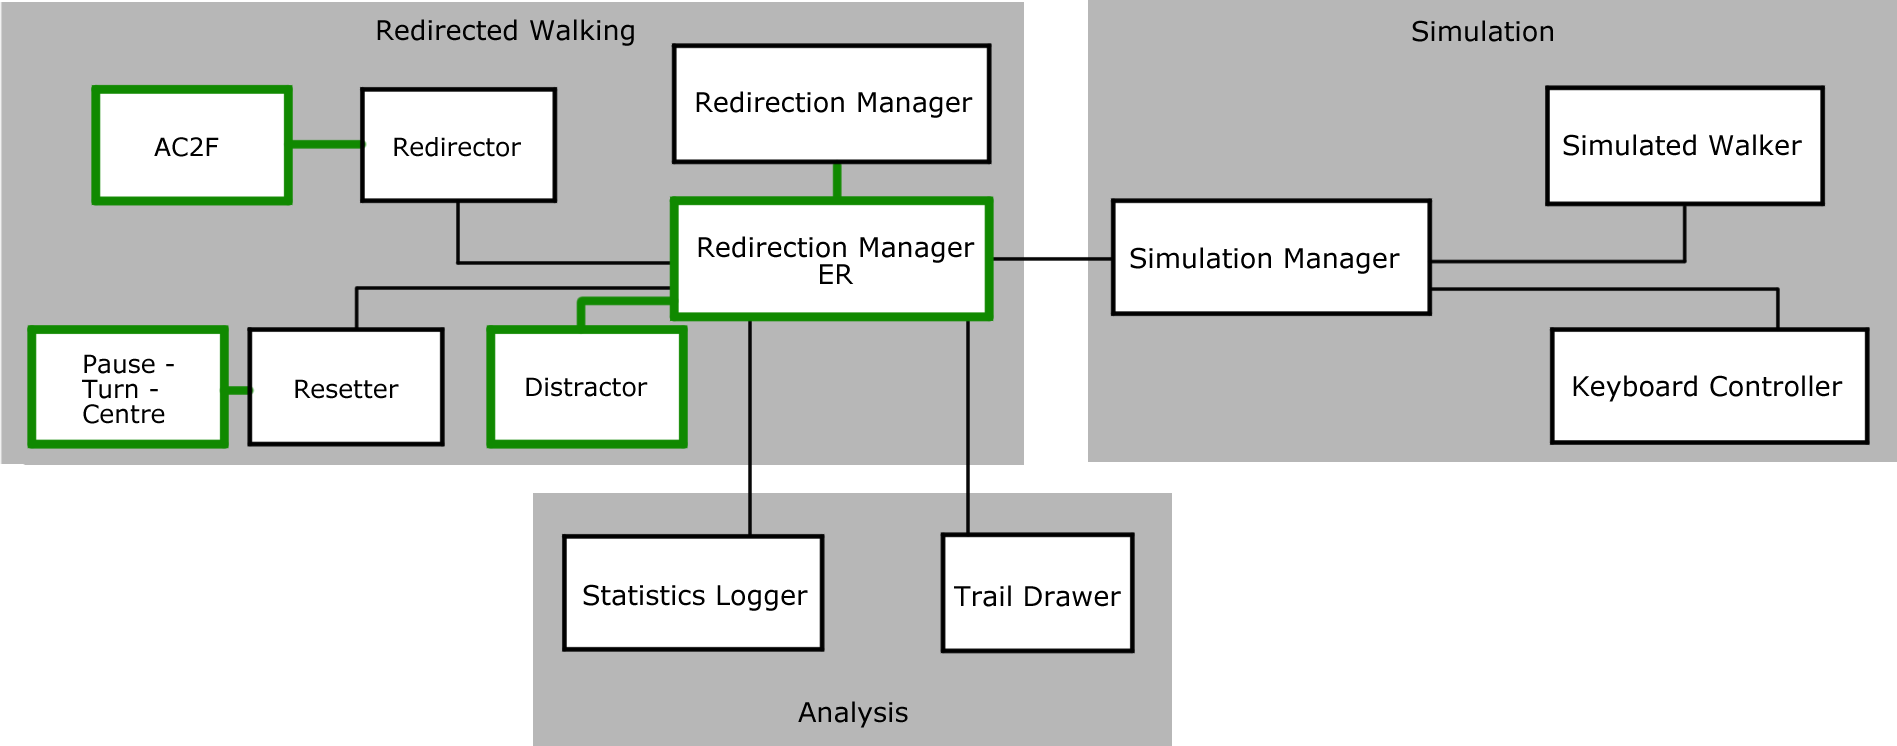
\includegraphics[width=1.0\textwidth]{figures/graphs/ToolkitExtension.png}
    \caption[Extended Structure of the Redirected Walking Toolkit]{This illustration provides an overview on how the structure of the redirected walking toolkit has been extended. New additions are marked with the use of green outlines. The original structure can be seen in Figure~\ref{fig:rdwToolkitStructure}.}
    \label{fig:rdwToolkitExtendedStructure}
\end{figure}

As part of developing Ensemble Retriever, Azmandian et al.'s Redirected Walking Toolkit~\cite{azmandian2016redirected} has been extended to support the usage of distractors and any other interfacing that the game has required. A chart showing the general additions to the toolkit's architecture can be found in Figure~\ref{fig:rdwToolkitExtendedStructure}. The general thought process throughout the development of these extensions was to not do any significant changes to the toolkit itself for the sake of keeping its modular structure. If functionality could be built on top of parts of the toolkit, then inheritance was used. If any part of the toolkit required major changes, it would be copied to a separate file which these modifications were written in. As far as minor changes are concerned, these mostly consisted of changing some data access properties of variables to allow for easier communication between classes or bug fixes.

To supplement the general overview in Figure~\ref{fig:rdwToolkitExtendedStructure}, the following list provides slightly more details on the exact extensions that have been implemented:
\begin{itemize}
    \item \lstinline{RedirectionManagerER} which extends \lstinline{RedirectionManager} to facilitate communication and management between new components.
    \item The ''Align Centre To Future'' (AC2F) Redirector. This redirector is aimed to be used while standing still.
    \item The ''Pause - Turn - Centre'' Resetter.
    \item The Distractor Trigger System.
    \item A \lstinline{ExperimentDataManager} script which handles data collection and experiment management.
    \item A \lstinline{GainIncrementer} script which is used as part of Experiment 1.
\end{itemize}

Each of these will be further detailed in the following sections. 

\section{Managing The Extended Architecture}
The \lstinline{RedirectionManagerER} script~\cite{redirectionManagerER} works in a similar way to the base class it extends. It facilitates communication between all of the new distractor related components and a few other things. These include switching between S2C and AC2F whenever distractors trigger, sampling position changes to calculate future walking directions, checking for alignment with future path during distractor battles and some additional debug related functionality. In this case, the manager makes use of two redirectors which consists of the S2C and AC2F redirectors. S2C is used when walking due to its rather generic nature, while AC2F is used during distractor battles as it is more specialised in terms of how it redirects.

Distractors in general function very similarly to resetters. They have associated callbacks and triggers which can generically be extended for whatever use the developer needs. They also have their own trigger safe bounds, which in general should happen somewhat earlier than what a reset would. It is necessary to keep in mind that once a distractor triggers, the user will need time to be able and stop walking without hitting the reset trigger bounds. The size of this buffer will mostly depend on the walking speed of users, but it is useful to try and find a balance in terms of the distance between these two bounds. The reasoning for this is that a large movable space before triggering any distractors would be preferable as they might trigger too often otherwise. This buffer was originally 0.5m, but has since been increased to 1m due to observations during Experiment 1.

\section{Distractor Enemies}
There is no directly generic script or class for distractors in the provided solution as there are very few strict guidelines on how these can be made. In general, \lstinline{RedirectionManagerER} stores a generic list of all potential distractor objects that can be spawned. Whenever the user reaches the distractor trigger bounds, the \lstinline{RedirectionManagerER} script will in this case spawn a distractor from its list.

A distractor's primary responsibility after being spawned is to notify the manager whenever it is finished so that the manager can call relevant callbacks and clean up after the distractor. Other than this, any behaviour could be programmed into the developed distractor. For Ensemble Retriever, all distractors extend a \lstinline{DistractorEnemy} script~\cite{distractorEnemyScript} which handles this responsibility in conjunction with some generic enemy behaviour. In a more general solution though, some generic base distractor class would likely be present.

\section{The ''Align Centre to Future'' Redirector}
\begin{figure}[htbp]
  \centering
  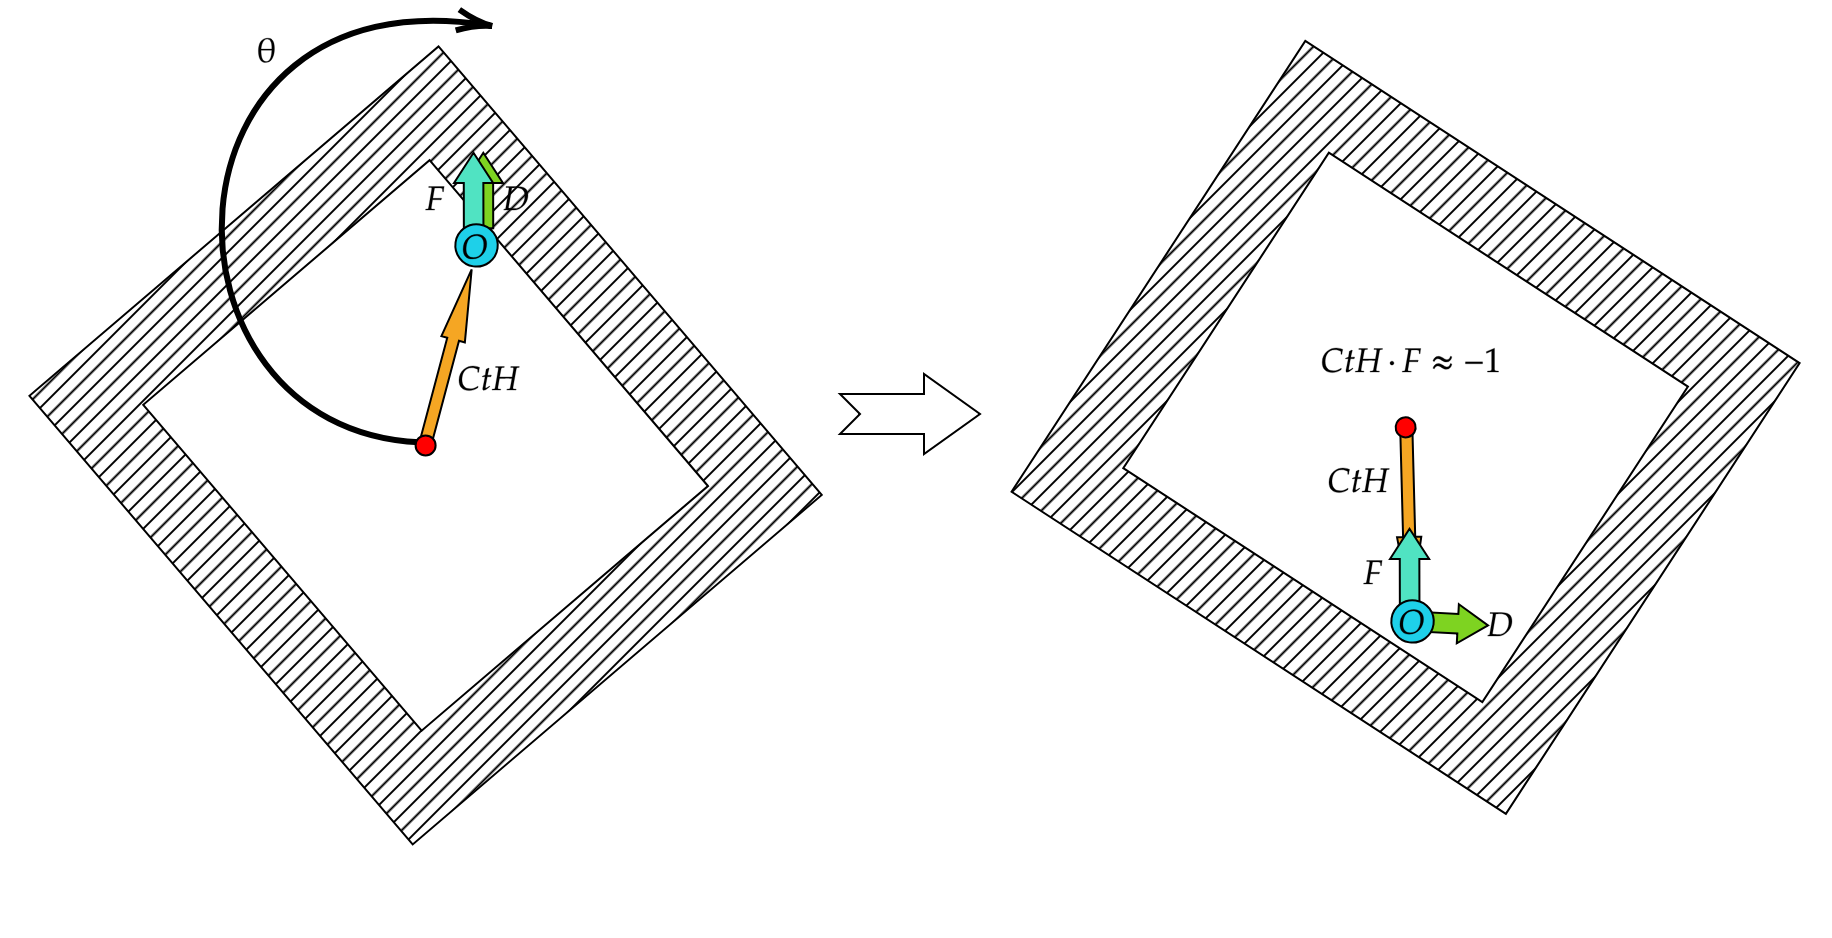
\includegraphics[width=\textwidth]{figures/graphs/AC2F.png}
  \caption[Align Centre to Future Algorithm Example]{AC2F aims to choose the rotation gains that bring the physical centre to head ($CtH$) vector in alignment with the future virtual walking direction ($F$) of the user. The user's current facing direction ($D$) is not used other than setting the value of $F$ as the algorithm starts. The origin of this reorientation is at the position of the user ($O$).}
  \label{fig:ac2f}
\end{figure}

The ''Align Centre to Future'' (shortened to AC2F) redirector is based on what Peck et al.~\cite{peck2010improved} as well as Chen and Fuchs~\cite{chen2017towards, chen2017supporting} have mentioned in terms of a modified future path driven S2C algorithm. Neither of their research provided any source code for how they modified S2C and as such, AC2F is loosely based on Azmandian et al.'s S2C implementation, which is part of the redirected walking toolkit. AC2F relies on rotation gains and an alignment heuristic to align the user's future virtual path towards. The definition of the user's future virtual path in this case consists of sampling the last second of their positional changes. The alignment heuristic on the other hand is the centre of the physical space. An illustrated view on how the algorithm works can be seen in Figure~\ref{fig:ac2f}. The algorithm aims to choose between negative or positive rotation gains in a way that results in closer alignment towards the heuristic. The source code for the algorithm can be found in the project repository~\cite{ac2fScript}.

\subsection{Algorithm Pseudocode}
The AC2F algorithm could roughly be summarised in the following simplified pseudocode:
\\
\begin{algorithmic}
\State chosenInjection = 0; \LineComment{Check if the change in rotation exceeds the threshold for applying gains}
\If {(deltaHeadRotationAngle >= rotationThreshold)}
    \State negativeRotationGainInjection = deltaHeadRotationAngle * negativeRotationGain;
    \State positiveRotationGainInjection = deltaHeadRotationAngle * positiveRotationGain;
    \State dotProductFromNegativeInjection = Dot(negativeRotationGainInjection * physicalCentreToHead, futureVirtualWalkingDirection);
    \State dotProductFromPositiveInjection = Dot(positiveRotationGainInjection * physicalCentreToHead, futureVirtualWalkingDirection);
    \If {(dotProductFromNegativeInjection < dotProductFromPositiveInjection)}
        \State chosenInjection = negativeRotationGainInjection;
    \Else
        \State chosenInjection = positiveRotationGainInjection;
    \EndIf
\EndIf
\State redirectionRoot.Inject(chosenInjection);
\end{algorithmic}

\vspace{0.3cm}
The gist of the algorithm is that it checks which of the two types of rotation gains that result in the best alignment towards the future virtual walking direction. In this case, dot products are compared with an alignment goal of \textasciitilde-1. This value is the dot product for when the user's future virtual path points in the opposite direction of a vector between the centre of the room and the user's head. Once a gain has been decided for use, it is injected to the root of the redirected walking hierarchy. The angle of this injection consists of the change in head rotation between two frames multiplied by the chosen gain.

Given that these calculations run every frame, it may not necessarily be the best solution in terms of performance. Despite this, the implementation was chosen to work this way for the sake of readability and simplicity as the performance cost was negligible. 

\subsubsection{Hypothetical Optimisation of AC2F}
In the hypothetical case of it being necessary to optimise AC2F, there are a few useful technicalities that could be considered. One of these is that the algorithm always will rotate the redirected walking root in either a clockwise or counterclockwise fashion depending on which of these takes the shortest time. Head rotations will also either be in a clockwise or counterclockwise direction. Applying a positive rotation gain to a head rotation will result in the redirected walking root to rotate in the same clockwise/counterclockwise direction. This effect means that the root will rotate slightly with the head rotation. Applying a negative rotation gain on the other hand will result in the opposite clock direction, meaning that the root will rotate slightly against head rotation. 

Given this behaviour, it is possible to skip dot product comparisons once the algorithm has decided whether to align in a clockwise or counterclockwise manner. In this case, there will always be a correct gain type to choose depending on which clock direction the head is rotating in.

\subsection{Smoothing}
One problem with rotation gains is that switching between positive and negative gains with large differences makes it very easy to notice redirection. This problem can be mitigated with the use of smoothing components which can be added to redirection algorithms. Particularly, smoothing can be applied by interpolating from a positive gain injection to a negative whenever this change is needed and vice versa. This interpolation creates a more subdued and gradual change rather than quickly jumping from one type of gain to the other. The main challenge with smoothing rotation is that we cannot interpolate the actual gains themselves as these have to stay static. Instead, we need to interpolate the camera injections that happen which will vary frame by frame depending on how much the user's head moves. As such, standard interpolation which has a set start and stop value is not possible as the stop/target value to interpolate towards will change every frame. Instead, the implementation AC2F uses was found on the Unity Forums~\cite{smoothingFormula} which is smoothing solved using a differential equation. The formula for this interpolation with the corresponding context is as follows:

$$
f = \frac{followerOldValue - targetOldValue + (targetNewValue - targetOldValue)}{(interpolationSpeed * t)}
$$
$$
followerNewValue = \frac{targetNewValue - (targetNewValue - targetOldValue)}{(interpolationSpeed * t) + f * Exp(-interpolationSpeed * t)}
$$
\begin{description}
    \item[followerOldValue:] The interpolated value this formula output during the prior frame.
    \item[followerNewValue:] The new interpolated result which this formula outputs during the current frame.
    \item[targetOldValue:] The value of the target during the prior frame. 
    \item[targetNewValue:] The value of the target during the current frame.
    \item[interpolationSpeed:] The speed of interpolation.
    \item[t:] Input interpolation time. This value is within the range of [0, 1]. 
    \item[f:] An intermediary variable to split up the equation.
\end{description}

Using this formula allows for smooth interpolation between rotation gain types even though the target may change slightly every frame. 

\subsubsection{Dealing With Edge Cases}
The AC2F algorithm makes use of a threshold for head rotations before applying any gains. The reason for this threshold is to avoid applying gains when the head is relatively still, but still moving due to small head vibrations and tracking inaccuracies. This threshold poses somewhat of a challenge in terms of how to deal with smoothing. If smoothing already is in progress and a head rotation goes below the threshold, then what should the algorithm do? One option would be to disable smoothing when this happens, but this creates an issue with a specific edge case. Whenever a user rotates with their body and head, the stopping motion results in a small bob towards the opposite direction. This small bob is below the threshold for applying gains and results in a somewhat jarring difference between applying gains and not applying them if we disable smoothing.

To deal with this edge case, AC2F allows the smoothing component to continue until it is finished. This approach deals with this specific edge case, but still has some problems of its own which could be improved in the future. If a user moves with only their head instead of head and body, then the smoothing will result in a somewhat sliding rotation effect when the user stops their head. While this effect only lasts for less than half a second, it could still be considered as annoying or unwanted. Fixing this problem while still also dealing with the prior mentioned edge case would be ideal in terms of smoothing. 

\section{The ''Pause - Turn - Centre'' Resetter}\label{sec:pauseturncentre}
\begin{figure}[htbp]
  \centering
  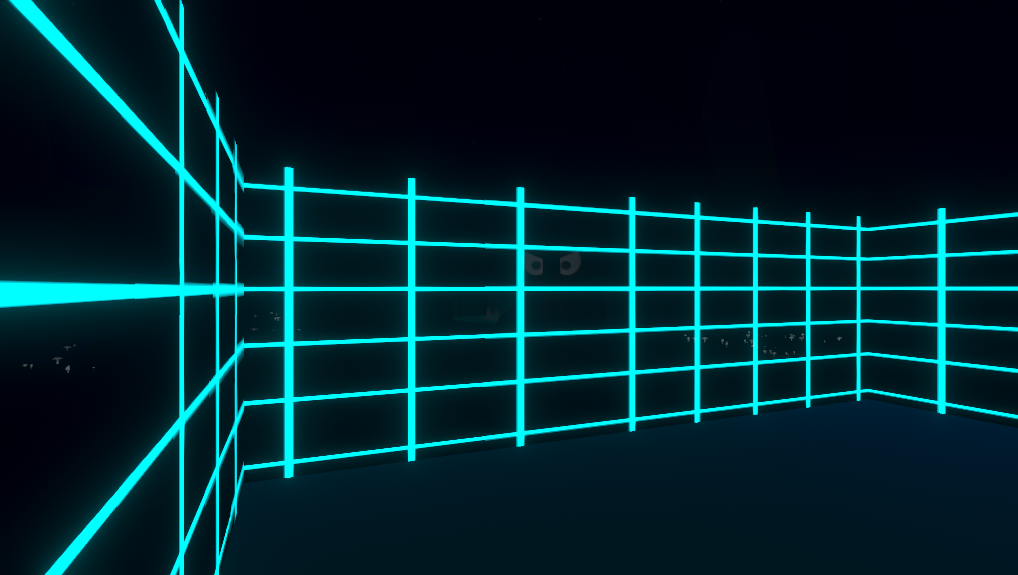
\includegraphics[width=0.5\textwidth]{figures/screenshots/pauseTurnCentreExample.png}
  \caption[Pause - Turn - Centre Screenshot]{This screenshot shows the Pause - Turn - Centre resetter in action. The virtual world has been mostly faded away and paused while the user can normally look around in the representation of their physical space.}
  \label{fig:pauseTurnCentreExample}
\end{figure}

As mentioned in Section~\ref{sec:choosingTheRightReset}, there are a variety of issues with current resetting techniques which limit their usefulness. To deal with these, a new resetter has been developed for this thesis which is called ''Pause - Turn - Centre''. This resetter takes inspiration from the Freeze - Turn resetter~\cite{williams2007exploring} as well as Sra et al.'s discussions on hiding noticeability through visibility limitation methods~\cite{sra2018vmotion}. The end result is somewhat different from Freeze - Turn with changes that aim to improve effectiveness and user experience. The source code for the resetter can be found in the project repository~\cite{pauseTurnCentre}.

Whenever the Pause - Turn - Centre resetter triggers, it will quickly fade in a chaperone style boundary which represents the physical space. At the same time, a slightly transparent black layer will be used to fade out the virtual environment so it is only slightly visible. While this resetter is active, a negative rotation gain of -1 is used to effectively freeze the y-rotation of the user in the virtual world. Meanwhile, the user can still look around in the representation of the physical space with normal head rotation. As the name implies, components of Ensemble Retriever that exist within the virtual world are paused until the resetter has finished. The resetter finishes when the user looks towards the centre of the physical space, meaning their walking direction will be towards its centre. A screenshot showing the resetter after being triggered can be seen in Figure~\ref{fig:pauseTurnCentreExample}.

The resulting behaviour avoids the issues that other resetters have in terms of cybersickness and sub-optimal reorientation. Cybersickness is minimised by obscuring the virtual world with a slightly transparent layer as vision limiting techniques decreases noticeability of redirection~\cite{sra2018vmotion}. It also allows the user to clearly see where the bounds of the physical space are. By instructing the user to look and move towards the centre of the room, there are no possibilities of becoming ''stuck'' between resets like when using 180-degree turns. The overall rotation that the user has to make is also smaller than 360 degrees, meaning that they will not be wrapped around any physical tethered cables which could cause issues. The trade-off for these improvements is the potential for this to be considered as more disruptive, but it could be argued that the improvements to safety, effectiveness and user comfort are worth this disruption.

\subsection{Clipping Related Problems}
\begin{figure}[htbp]
  \centering
  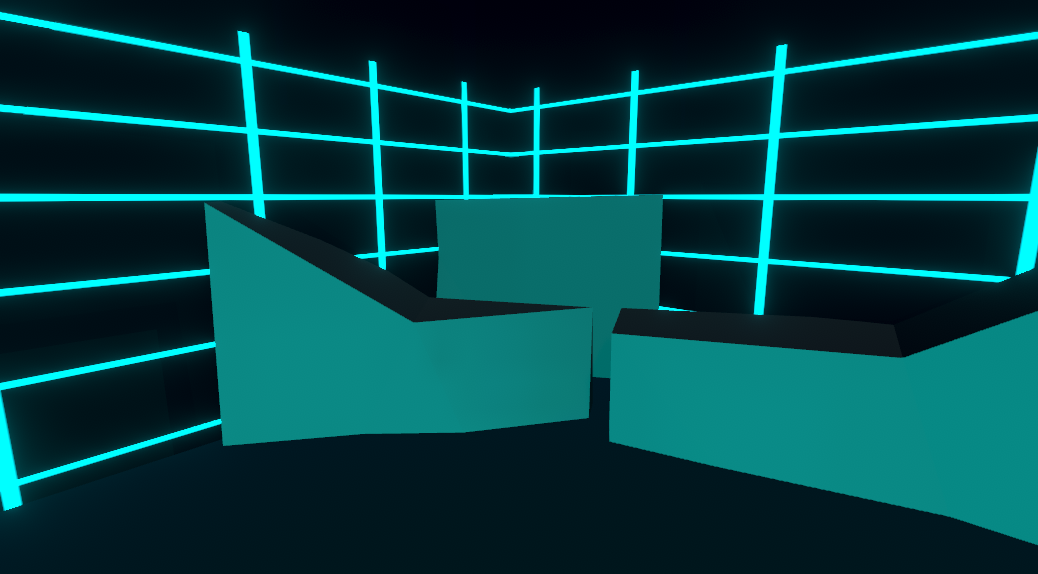
\includegraphics[width=0.5\textwidth]{figures/screenshots/pauseTurnCentreClipping.png}
  \caption[Pause - Turn - Centre Clipping Bug Screenshot]{This screenshot shows a prior bug that existed when using the Pause - Turn - Centre resetter. Virtual world geometry has in this case clipped into the representation of the physical space, resulting in rather confusing visuals as the virtual world is effectively paused during this time.}
  \label{fig:pauseTurnCentreClippingBug}
\end{figure}

One issue that cropped up during the implementation of Pause - Turn - Centre can be seen in Figure~\ref{fig:pauseTurnCentreClippingBug}. If the representation of the physical space overlaps with other geometry from the virtual world, then this would cause some rather confusing visuals. This confusion stems from the issue that a negative rotation gain of -1 is fully visible for this overlapping geometry. This problem has been solved in the following manner.

Two separate cameras are employed. One of these renders the virtual world while the other renders everything that exists under the redirected walking root and could be considered as the physical space. By forcing the depth level of the physical space camera to always be closest, we can draw the physical space representation over everything else that exists in the virtual world. As such, even if geometry overlaps into the physical space, this can not be seen as the physical space representation will be drawn on top of it. This solution has a benefit and a drawback. It is simple to implement as forcing one camera to render on top of another is as simple as setting a depth value for the camera itself. The downside is that using multiple cameras in VR is rather performance costly as each camera must render twice for stereoscopic vision. As such, there are effectively four render cameras in use instead of two. This approach becomes a larger performance problem with post-processing as this needs to apply to each camera. Despite this overhead increase, there is some granularity as the post-processing effects that are used can be tweaked for each individual camera. By doing so, it is possible to optimise away certain post-processing effects from the rendering of the physical space representation as it will not be seen very often. 

\subsection{Pausing the Game Using ''Pause - Turn - Centre''}
In order to properly pause relevant game objects in Ensemble Retriever with ''Pause - Turn - Centre'', it is necessary to define what is and is not pausable. This definition is solved by having all pausable dynamic objects extend a \lstinline{Pausable} class. By doing so, each dynamic object acquires access to some callbacks and pause state information. Pausing all pausables is handled by the \lstinline{RedirectionManagerER} script where it generates a list of all \lstinline{Pausable} objects and triggers a related pause callback for these. It is then up to each individual \lstinline{Pausable} object to control their paused behaviour. This approach allows for selective pausing of virtual world objects while allowing elements like the physical space representation and HMD tracking to still function. 
 
\section{Experiment Management}
The experiments that have been conducted for this thesis are managed through two primary scripts: \lstinline{ExperimentDataManager}~\cite{experimentDataManager} and \lstinline{GainIncrementer}~\cite{gainIncrementer}. The \lstinline{ExperimentDataManager} script takes care of all related data recording for Experiment 1 and 2 while the \lstinline{GainIncrementer} script is used during Experiment 1 to incrementally and randomly increase gains. Further details on what and how data was recorded can be seen in Chapter~\ref{chap:ex1} and~\ref{chap:ex2} for Experiment 1 and 2 respectively. 

\section{Supporting the y-axis in the Redirected Walking Toolkit}
As part of triggering relevant resets and other colliders, the redirected walking toolkit makes use of a ''head follower'' collider~\cite{headFollower} which represents the collider for the user's body. It will continuously be below the user's head position as the user moves around. One issue that was uncovered during development was that this functionality stopped working as intended if the redirected walking root changed y position. The reason for this is that the ''head follower'' collider did not take these changes into account and continuously attempted to place itself at a y-value of 0 in world space. This approach was not particularly flexible and as such, this functionality of the toolkit has been updated to support the y-axis. This improvement is handled by having the collider place itself at a local position of 0 rather than in world space, meaning that it will always be below the user due to the transformation hierarchy it exists in. 

\section{Game Design Overview of Ensemble Retriever} 
\begin{figure}[tbph]
    \centering
    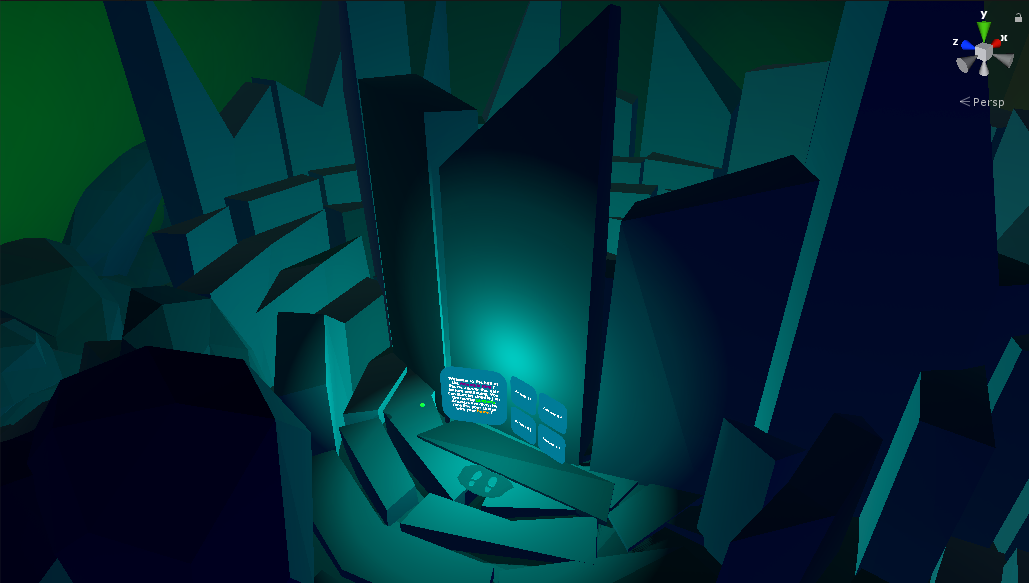
\includegraphics[width=0.8\textwidth]{figures/screenshots/HallOfTheMountainKingKindaLowRes.png}
    \caption[Screenshot of the ''Hall of The Mountain King'']{This screenshot from the Unity scene view shows the ''Hall of The Mountain King'' with the quiz section that the player has to answer.}
    \label{fig:mkhallWithWall}
\end{figure}

\begin{figure}[tbph]
    \centering
    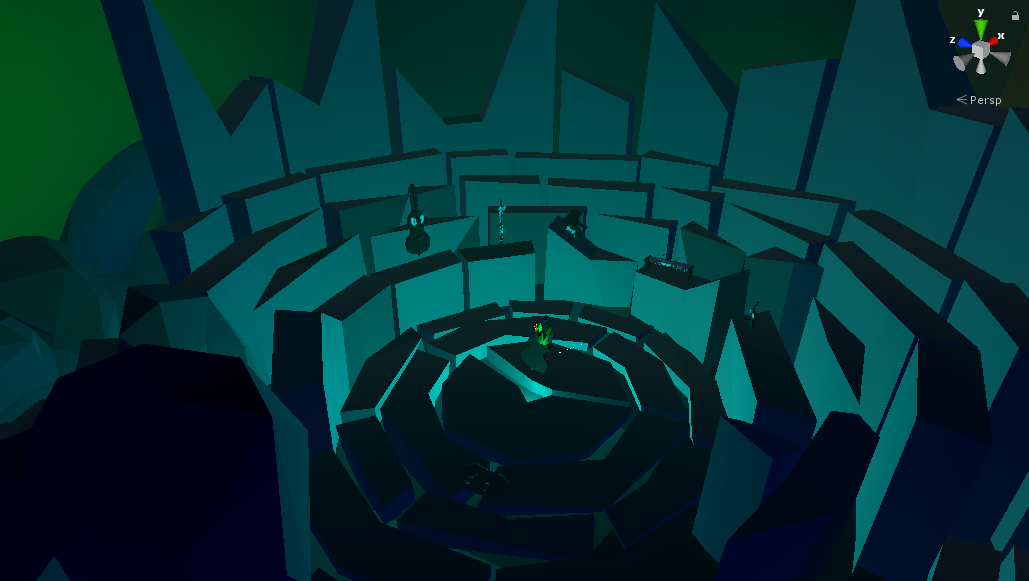
\includegraphics[width=0.8\textwidth]{figures/screenshots/HallOfTheMountainKing2KindaLowRes.png}
    \caption[Screenshot of the ''Hall of The Mountain King'' Without the Quiz Wall]{This screenshot from the Unity scene view shows the ''Hall of The Mountain King'' after the player has answered the quiz section in the game. This is where the Mountain King is fought.}
    \label{fig:mkhallWithoutWall}
\end{figure}
In Ensemble Retriever, the player takes the role of a conductor whose goal is to retrieve the ''Mountain King'', which is an instrument that has disappeared from their ensemble. In order to find the ''Mountain King'', the player has to walk around in a large virtual environment and ask the local residents for clues before they can enter the ''Hall of The Mountain King'' seen in Figure~\ref{fig:mkhallWithWall} and \ref{fig:mkhallWithoutWall}. Throughout the player's exploration of the virtual world, they are attacked by various distractor enemies which have to be defeated to gain experience points and progress the game. These battles consist of having the player use their contrabass shield to absorb enemy projectiles. Once enough projectiles have been absorbed, the player can counterattack with their magical conductor baton. Defeating distractors allows the player to level up over time and choose whether to upgrade their shield size or baton damage. The game culminates with a battle against the ''Mountain King'' that tests the player's skill and abilities which they have trained throughout their battles with distractor enemies.  

The following sections provide a more detailed context on the game itself and how distractors have been fully integrated into the experience.

\subsection{Virtual Environment}
\begin{figure}[tbph]
    \centering
    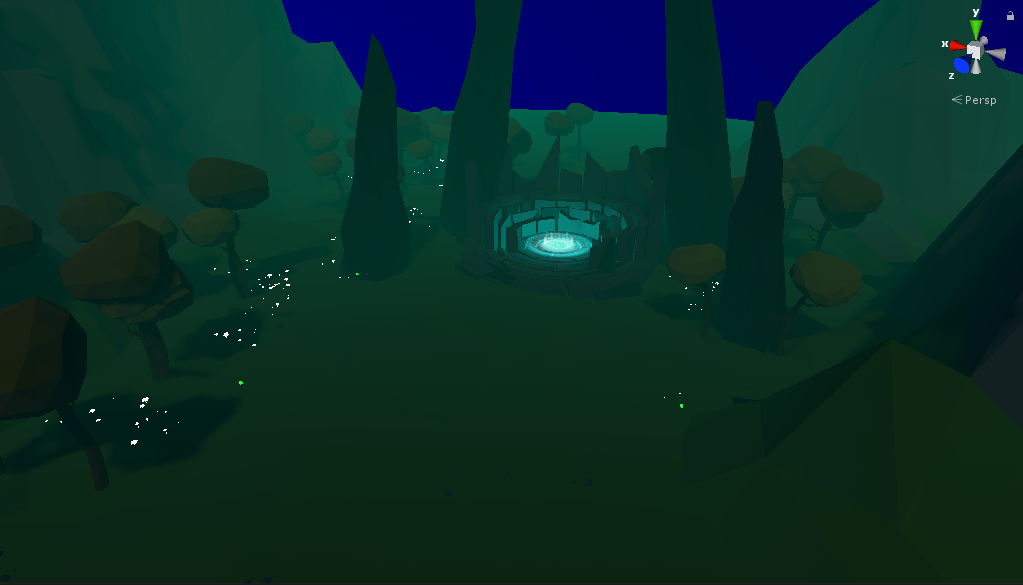
\includegraphics[width=0.8\textwidth]{figures/screenshots/EnvironmentKindaLowRes.png}
    \caption[Screenshot of the Environment in Ensemble Retriever]{This screenshot from the Unity scene view shows the virtual environment of Ensemble Retriever.}
    \label{fig:ensembleRetrieverEnvironment}
\end{figure}

\begin{figure}[tbph]
    \centering
    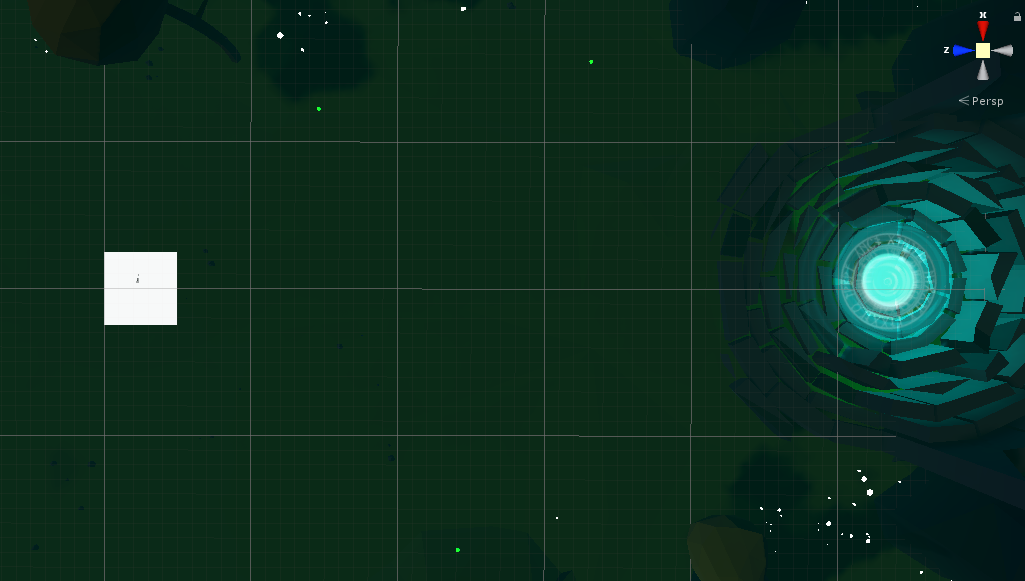
\includegraphics[width=0.8\textwidth]{figures/screenshots/TopDownExperiment1Spawn.png}
    \caption[Top Down Screenshot of Virtual Space That Players Walked Through]{This top-down screenshot of the environment shows the walkable area that players walked through in Experiment 1. In this case, players started where the white square representing the physical space is and moved to the portal on the right. On their path, they had to visit three small green fireflies. It should be noted that each small square in the grid is equivalent to 1m squares in real life.}
    \label{fig:topDownViewOfEnvironment}
\end{figure}

The virtual environment that players walked through can be seen in Figure~\ref{fig:ensembleRetrieverEnvironment}. A top-down view is also available in Figure~\ref{fig:topDownViewOfEnvironment}. If taking a straight line from the start to the end, players would need to walk \textasciitilde55m, although the actual distance is a bit longer as visiting the three fireflies also was necessary. 

\subsection{Game Flow}
This section provides an outline of the flow of Ensemble Retriever and how the game progresses throughout a play session. 

\begin{figure}[tbph]
    \centering
    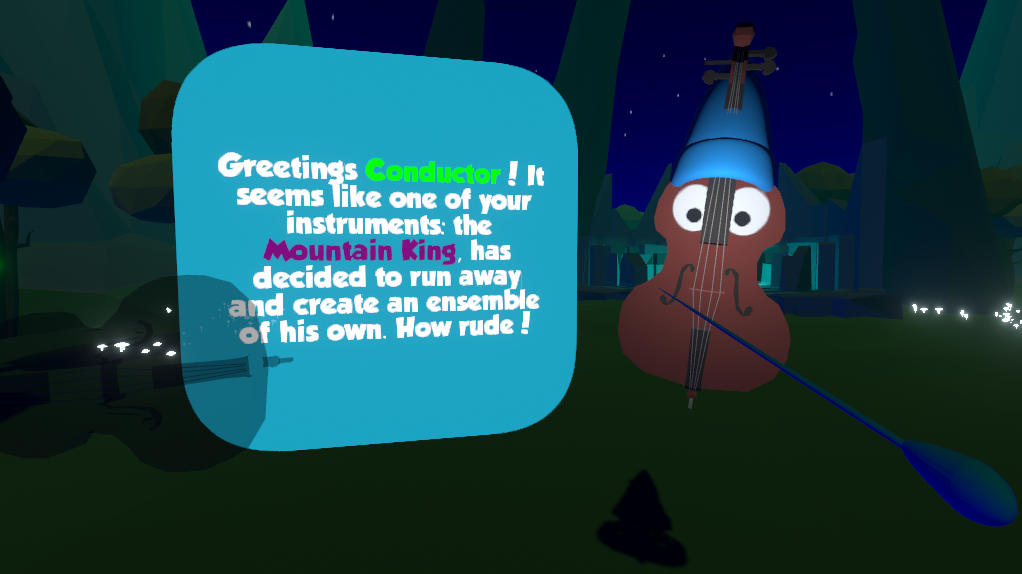
\includegraphics[width=0.8\textwidth]{figures/screenshots/Tutorial.png}
    \caption[Screenshot of the Tutorial in Ensemble Retriever]{This screenshot from Ensemble Retriever illustrates the tutorial that one of the ingame characters gives to the player.}
    \label{fig:tutorial}
\end{figure}

Ensemble Retriever starts with a tutorial that teaches the player the basics of the game. As seen in Figure~\ref{fig:tutorial}, the tutorial is provided to the player by one of the ingame characters. It provides information on the context/story, the player's goal, how to deal with resets, how to fight enemies and what to do if they are lost. In Experiment 1, the tutorial also provides information on what the player should do if they notice they are being redirected. The entire tutorial is voiced in case the text is not sufficiently readable.

After the tutorial is finished, the game transitions to a walking phase where the player tries to reach the ''Hall of The Mountain King'' while being encouraged to visit three green fireflies that provide hints which will be relevant for a later part of the game. As the player walks around in this phase, distractor enemies will appear once they hit the maximum safe distance away from the centre. These enemies need to be defeated to progress and award experience points that the player can use to either upgrade the size of their contrabass shield or the damage that their conducting baton does. It should be noted that the fireflies fade away during battles to prevent their salience from potentially affecting the attention of the player since this could result in lower concentration~\cite{sitzmann2018saliency}. The walking phase of Ensemble Retriever is finished once the player enters the portal to the ''Hall of The Mountain King''. 

Once the player enters the ''Hall of The Mountain King'', any redirection gains are disabled. The reasoning for disabling gains is to allow the player to spend the last few minutes of the game getting used to normal head rotations before taking off the HMD. Inside the hall, the player has to answer a multiple choice quiz which asks questions based on the previous hints that could have been acquired from fireflies in the walking phase. The quiz itself cannot be failed, but the final score that the player is given ties with how many correct answers they give. The quiz itself has three questions in total.

Once the quiz is finished, the player will have to fight against the ''Mountain King''. This is a longer battle where the ''Mountain King'' will use combinations of all previous attacks that distractor enemies have been using to challenge the player. Once the ''Mountain King'' has been defeated, the game is finished and the player will be shown their scores which consists of four components:
\begin{enumerate}
    \item Time Score (How long it took to finish the game. Shorter times means higher scores).
    \item Damage Score (How much damage the player has taken in total. Less damage means higher scores).
    \item Quiz Score (How many correct quiz answers the player has gotten).
    \item Total Score.
\end{enumerate}

A full playthrough of Ensemble Retriever by the author can be seen on YouTube~\cite{ERPlaythrough} for further illustration.

\section{Fully Integrating Distractors with Game Mechanics}
\begin{figure}[tbph]
    \centering
    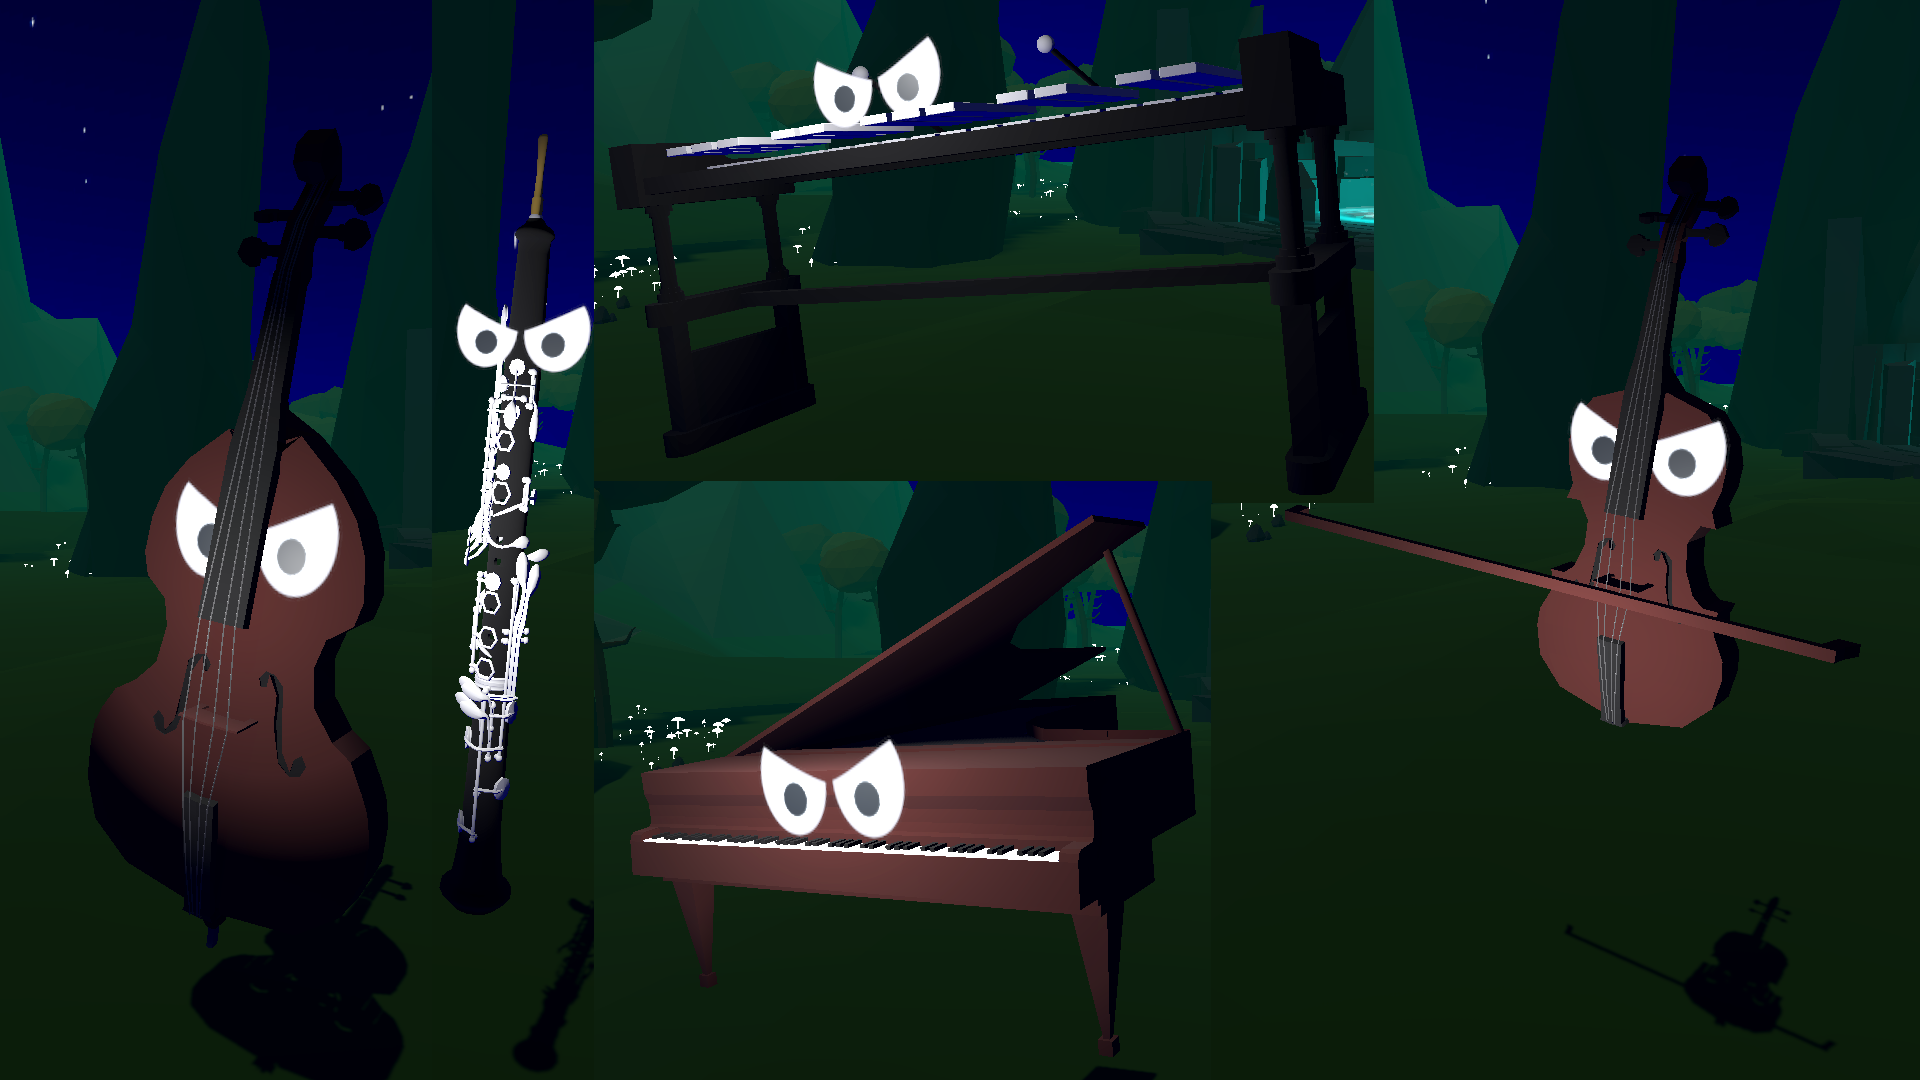
\includegraphics[width=1\textwidth]{figures/screenshots/Distractors.png}
    \caption[The Distractors of Ensemble Retriever]{These are the five distractor enemies that are employed in the Ensemble Retriever game.}
    \label{fig:allDistractors}
\end{figure}

The development resource budget of Ensemble Retriever was reasonably small (\textasciitilde1.25 months). As such, in order to have a reasonable scope and allowing for as much code/asset reuse as possible, the main mechanic that was decided to fully integrate with distractors was the enemy encounters in the game. Since the AC2F algorithm relies on rotation gains, the goal of using distractors in this case was to make the player move their head around as much as possible. Ensemble Retriever currently consists of five enemy distractors which can be seen in Figure~\ref{fig:allDistractors}. If we look back to the taxonomy of distractors which was presented in Section~\ref{sec:distractorTaxonomy}, these can be considered as explicit, concrete distractors that are fully integrated into the experience. In this case, the distractors are considered explicit as the player is told they have to fight them. 

From a game design point of view, their use can be seen as ''random'' enemy encounters which is a common mechanic in role-playing games. Instead of being random though, these enemy encounters trigger once the player has reached the maximum safe distance away from the centre of their physical tracking space. 

Once an enemy encounter starts, one of the five possible distractors is randomly chosen from a list. The chosen distractor is then removed from this list so it cannot be chosen again for some time. Once all distractor enemies have been chosen from the list, it is then repopulated with all five again. In the worst case scenario, this means that the same distractor might show up as the next enemy right after the list has been repopulated. The rationale for this approach is to avoid situations where the same distractor can show up too many times in a short space of time, potentially annoying the player due to limited variety as mentioned by Sra et al.~\cite{sra2018vmotion}. 

Each of the five distractor enemies rely on projectile attacks that have three potential movement speeds as well as a unique property per type of distractor. Before attacking, the distractor will make use of two telegraphs: one for the type of projectile it will attack with and one for how fast it will be. These telegraphs make use of both animation and audio cues, allowing the player to learn and identify the different types of attacks that are used so they can prepare accordingly. 

A standard enemy encounter consists of two phases: a tutorial phase and a proper battle phase. During the tutorial phase, the distractor will use its different attacks in order to teach the player its capabilities. In this phase, the distractor will not move away from its initial position. Once the player manages to counterattack the distractor, the real battle begins. During the battle phase, the distractor will randomly choose an angle between -360 and 360 degrees from the player after each attack, and rotate around them. The attack order will at this point also either be random or predetermined depending on the type of distractor. These approaches force a fair amount of head rotation from the player as they need to keep track of where the distractor moves and where their projectile attacks are. Furthermore, these approaches also makes good use of the full 360-degree space that virtual reality allows while providing many opportunities for applying rotation gains.    

The following sections will describe and detail each distractor that exists in Ensemble Retriever. It should be noted that the screenshots of these were taken from the debug mode of the game, hence why the conductor baton and shield are in fixed screen positions.

\subsection{The Contrabass}
\begin{figure}[tbph]
    \centering
    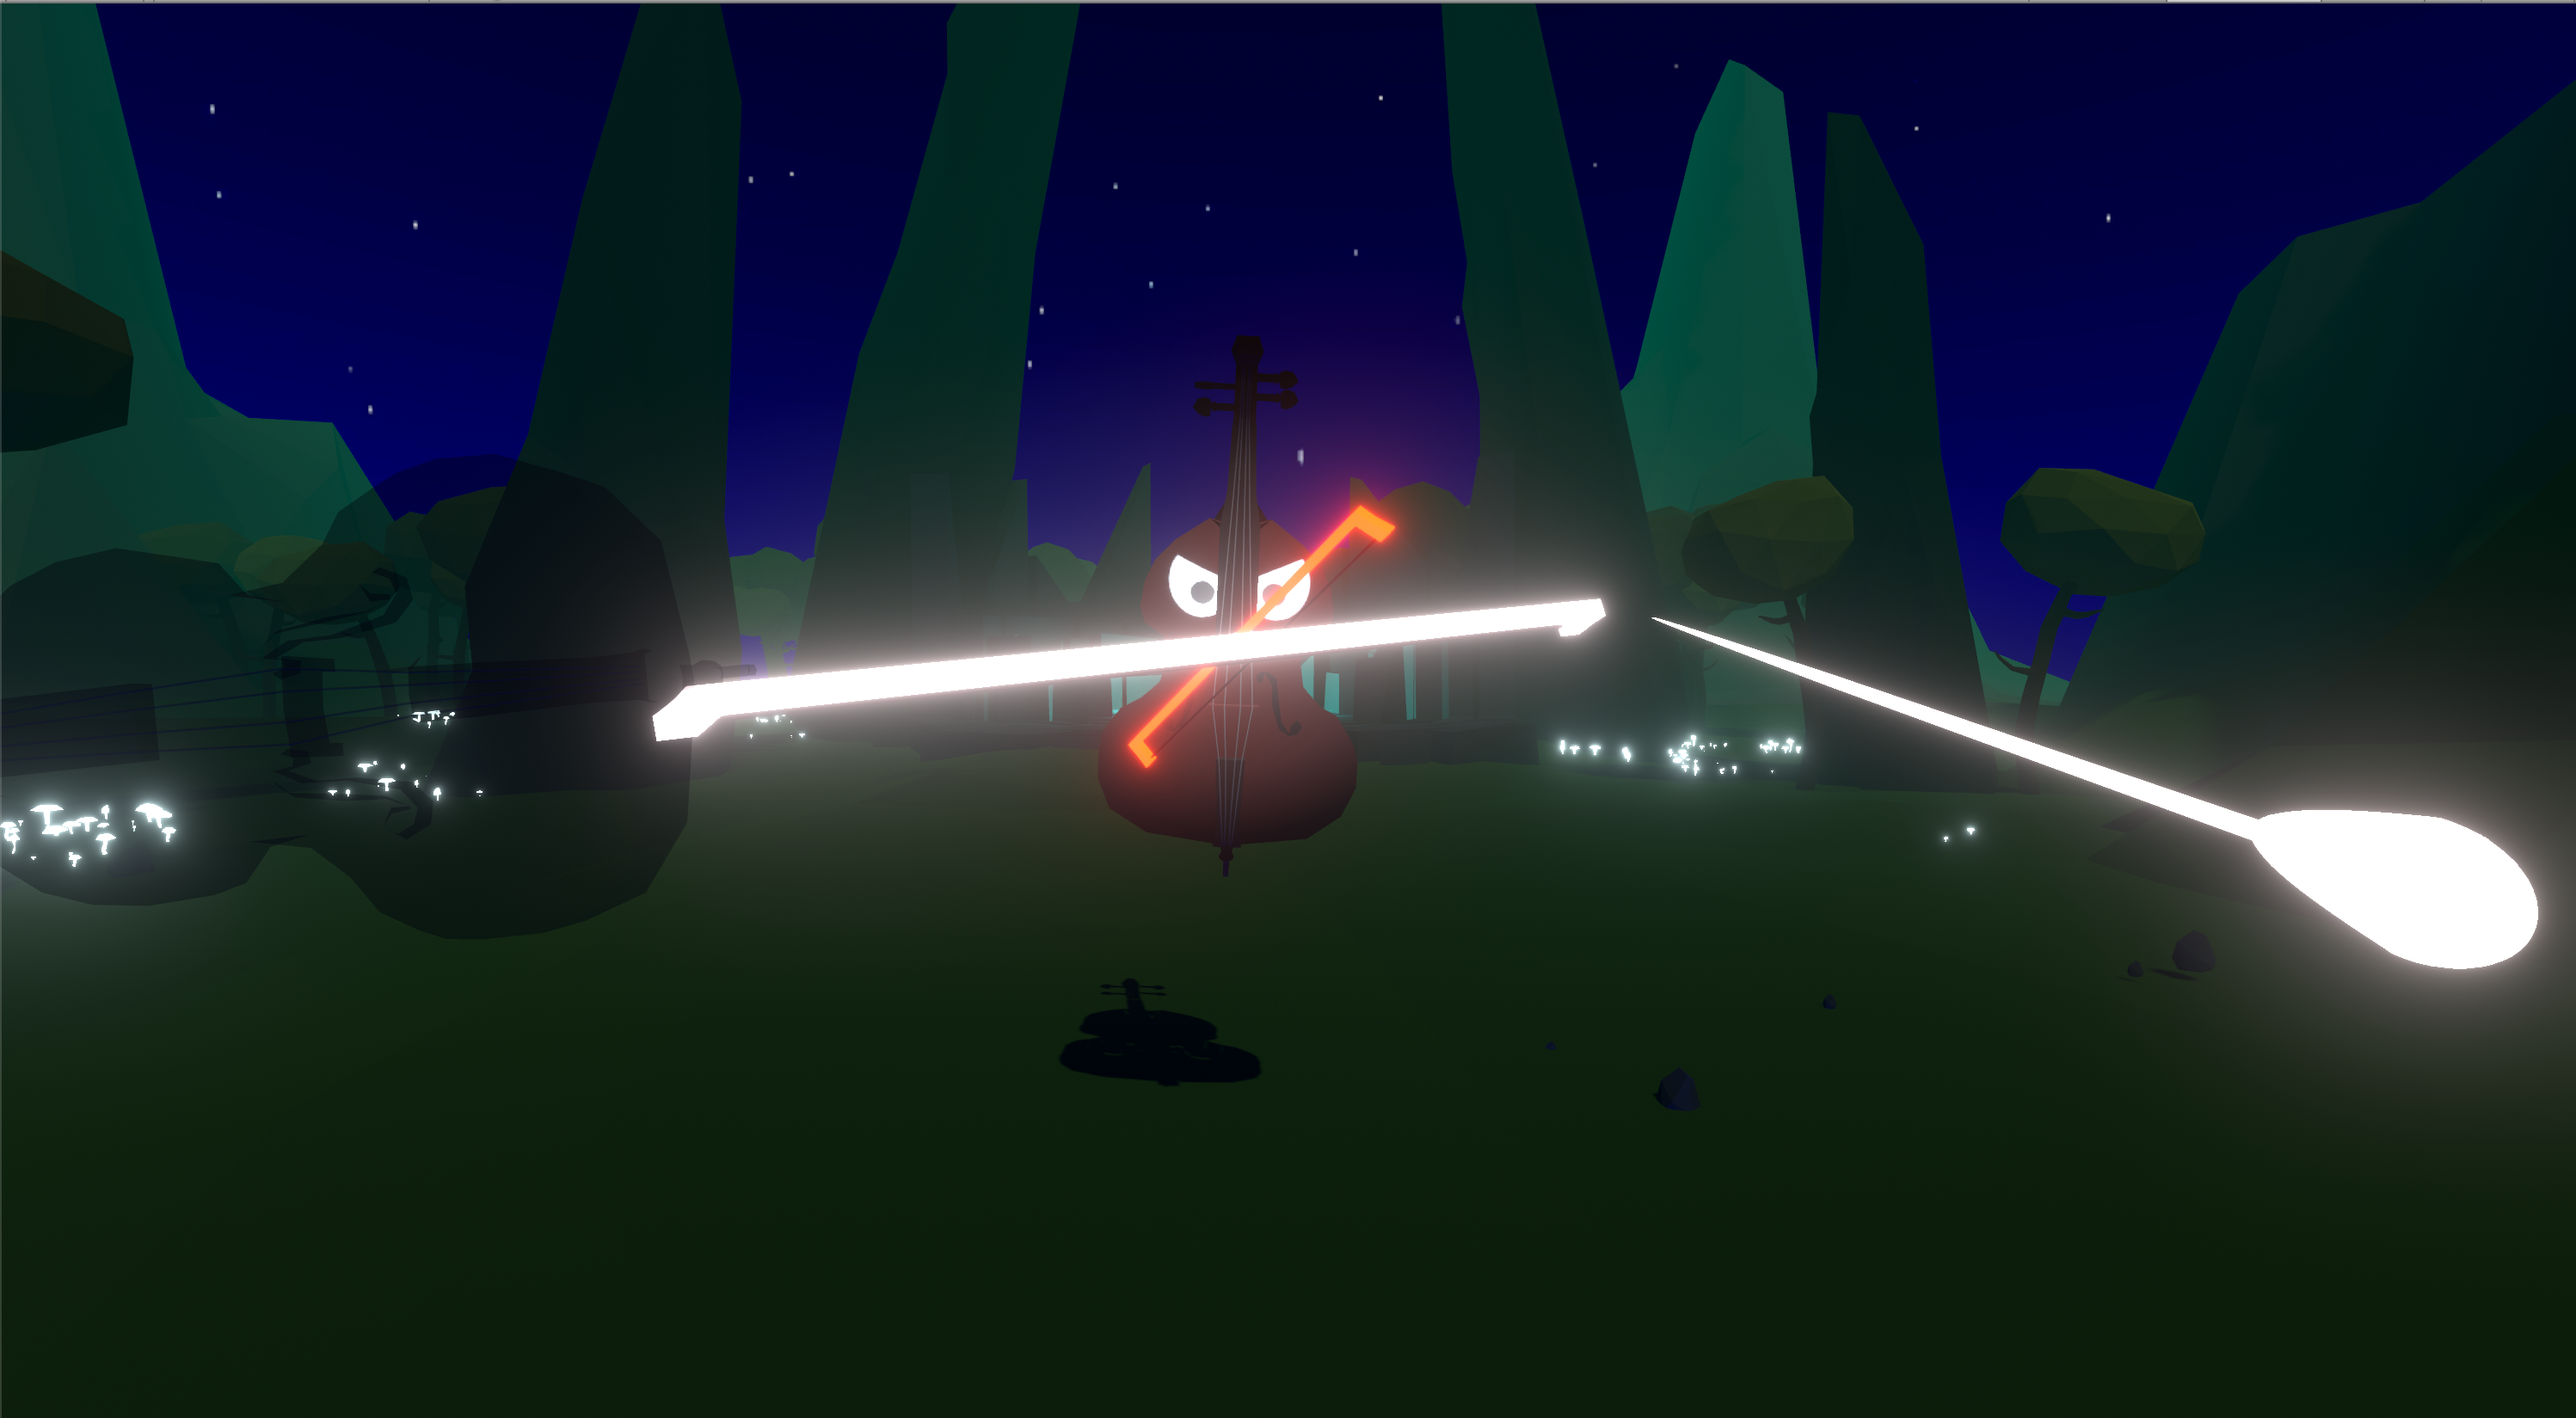
\includegraphics[width=0.75\textwidth]{figures/screenshots/contrabass.png}
    \caption[The Contrabass Distractor]{This screenshot shows off the contrabass distractor and its projectile attacks which travel directly towards the player.}
    \label{fig:contrabassDistractor}
\end{figure}
The first among the five distractor enemies is also the simplest one: ''The Contrabass'', as seen in Figure~\ref{fig:contrabassDistractor}. It attacks the player with projectiles that move towards them in a straight line. As a means to make the player move their head around more, the contrabass will mix slow and fast projectiles. A fast projectile will in this case move fast enough that it hits the player before a previously thrown slow projectile. This way, the player has to keep track of where the contrabass itself is when it uses fast projectiles while trying to remember where the slower moving ones are so they can absorb these as they come close. 
 
\subsection{The Oboe}
\begin{figure}[tbph]
    \centering
    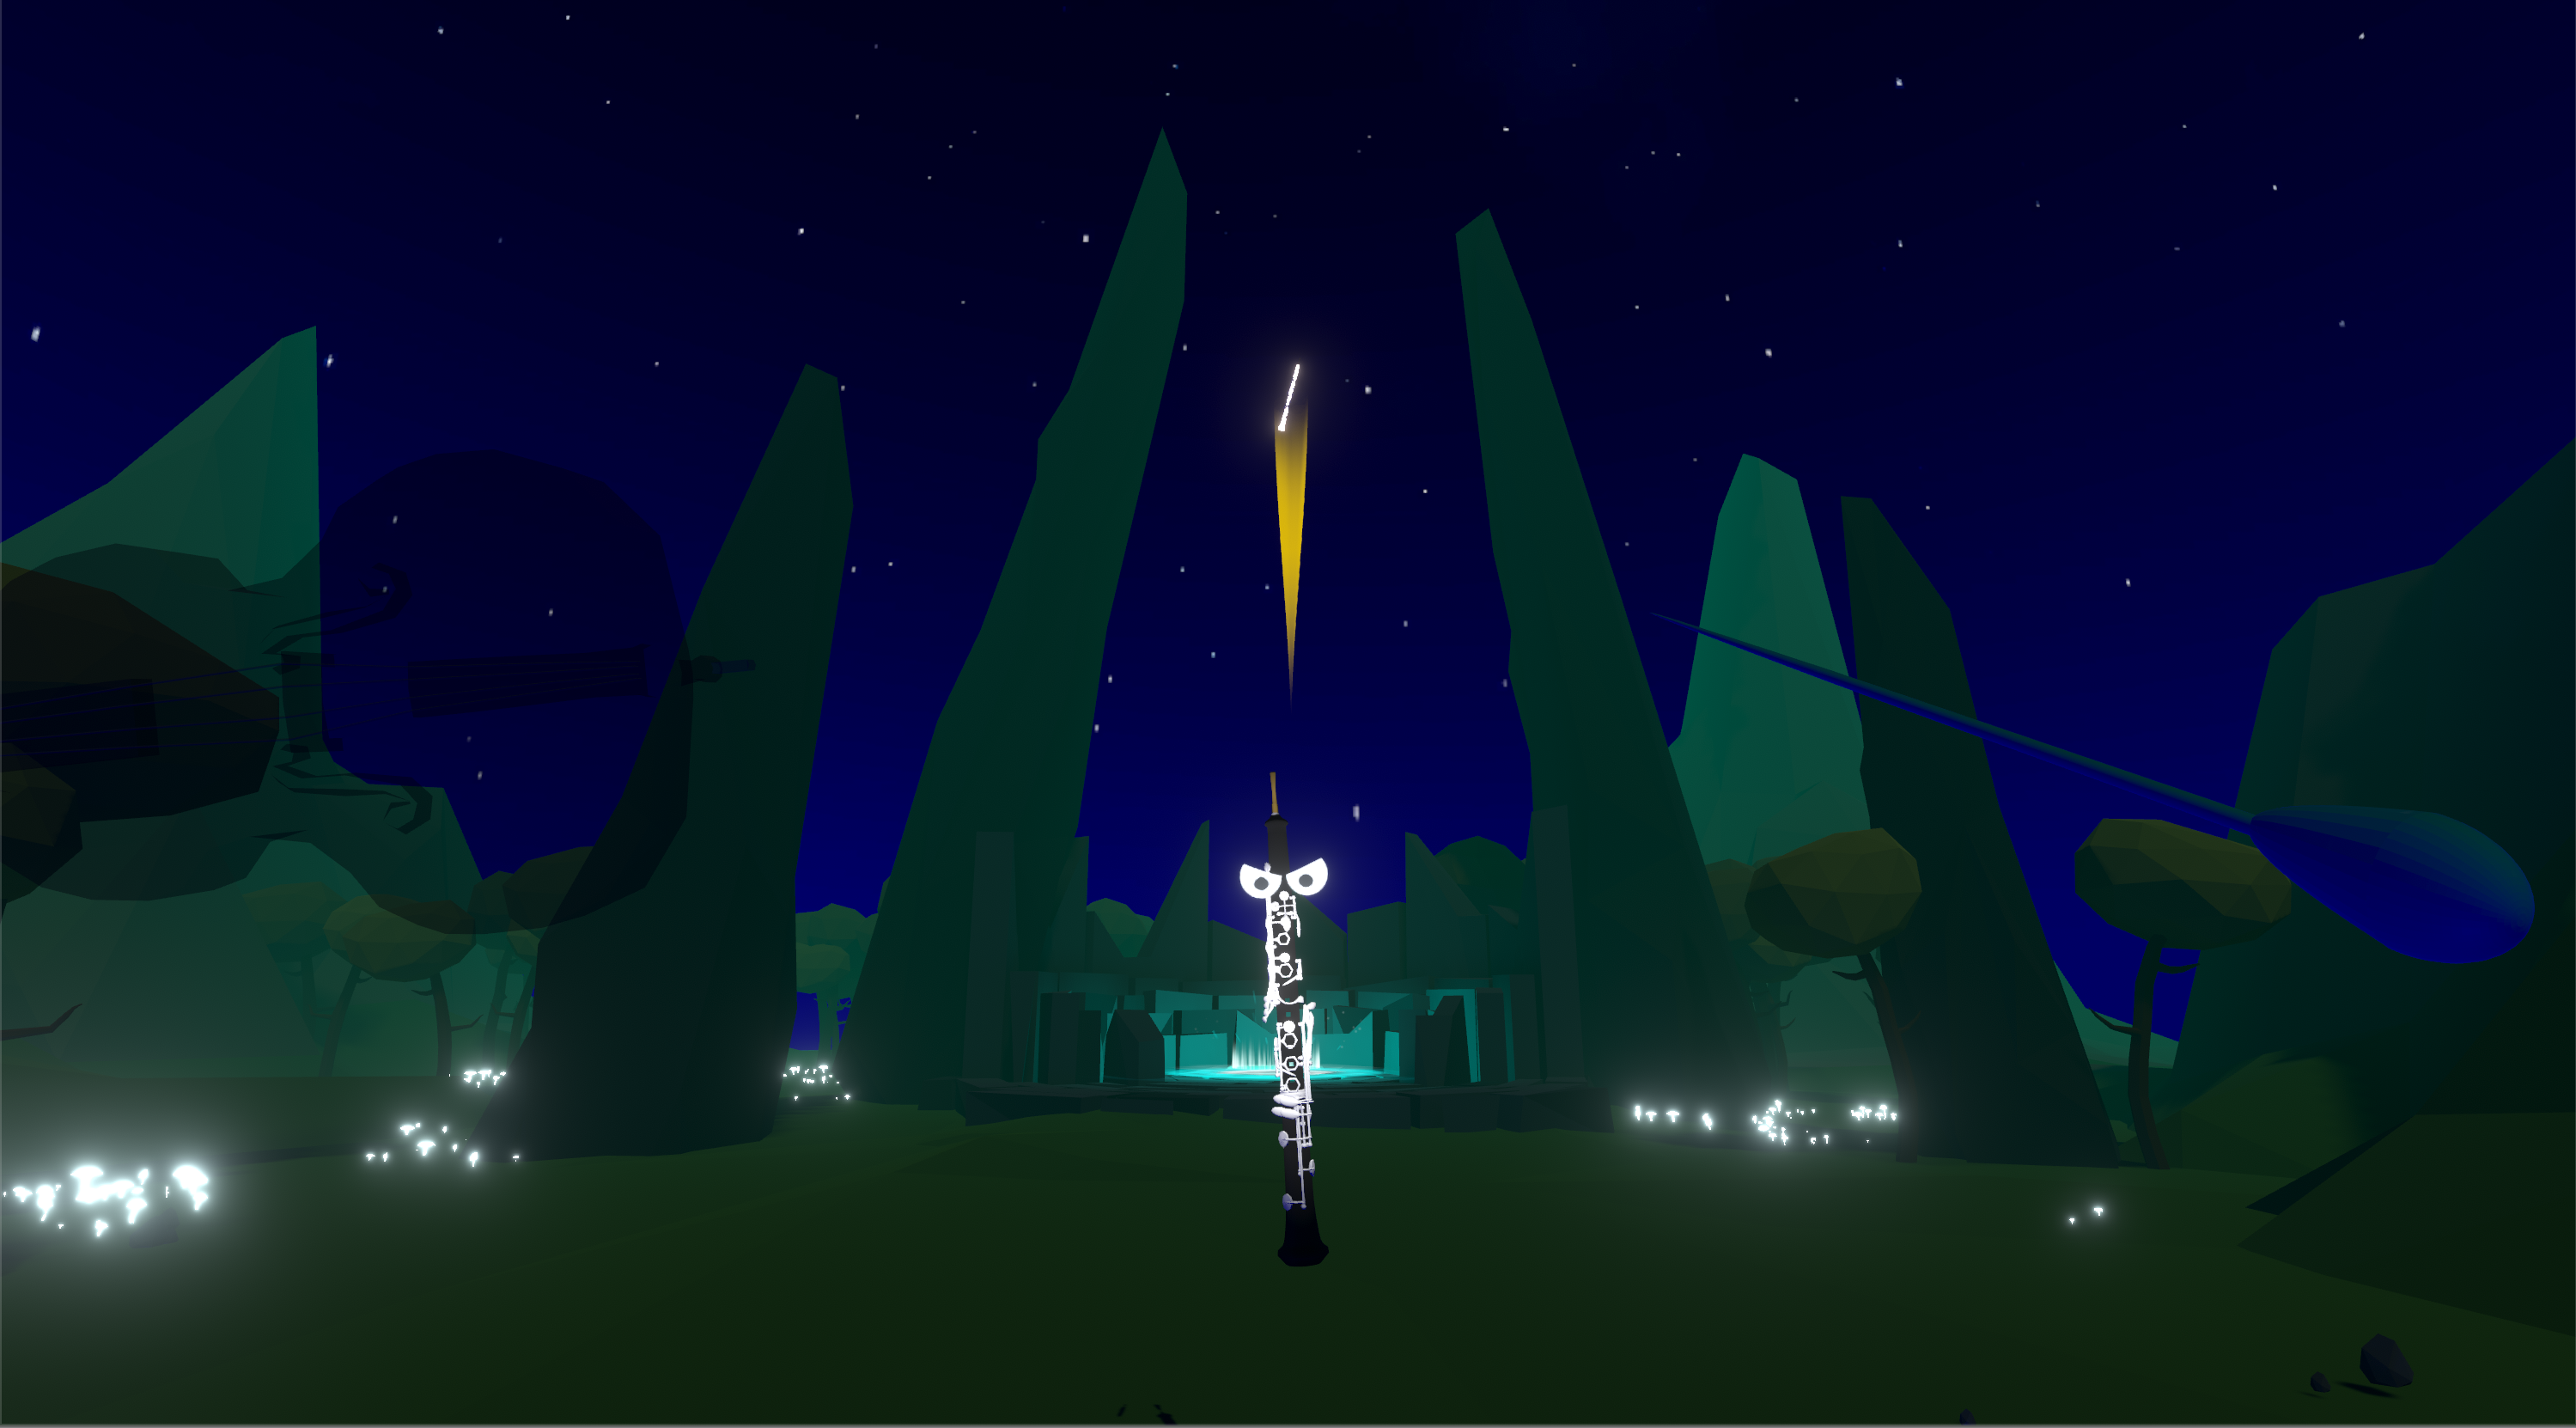
\includegraphics[width=0.75\textwidth]{figures/screenshots/oboe.png}
    \caption[The Oboe Distractor]{This screenshot shows the oboe distractor and its projectile attack which will travel on a vertical arc above the head of the player.}
    \label{fig:oboeDistractor}
\end{figure}

\begin{figure}[htbp]
  \centering
  \includesvg[width=0.5\textwidth]{figures/svgs/oboeProjectile.svg}
  \caption[Sideways 2D Example of Oboe Projectile Path]{An illustrated, sideways 2D example of how the oboe projectile travels. The blue circle and quad represents the player while the red circle represents the distractor that is about to attack.}
  \label{fig:oboeProjectile}
\end{figure}
The next distractor is ''The Oboe',' which can be seen in Figure~\ref{fig:oboeDistractor}. It attacks the player with projectiles that move in a vertical, 180-degree arc above the player's head before travelling straight towards their head. A rough two-dimensional figure illustrating this can be found in Figure~\ref{fig:oboeProjectile}. The Oboe attempts to facilitate head rotation by trying to hit the player from behind with projectiles. A clever player might end up holding the shield behind their head to absorb these, lessening the impact of the approach though. Despite this, it is still necessary to keep track of the projectiles as the Oboe moves and rotates around the player. 

\subsection{The Harpsichord}
\begin{figure}[tbph]
    \centering
    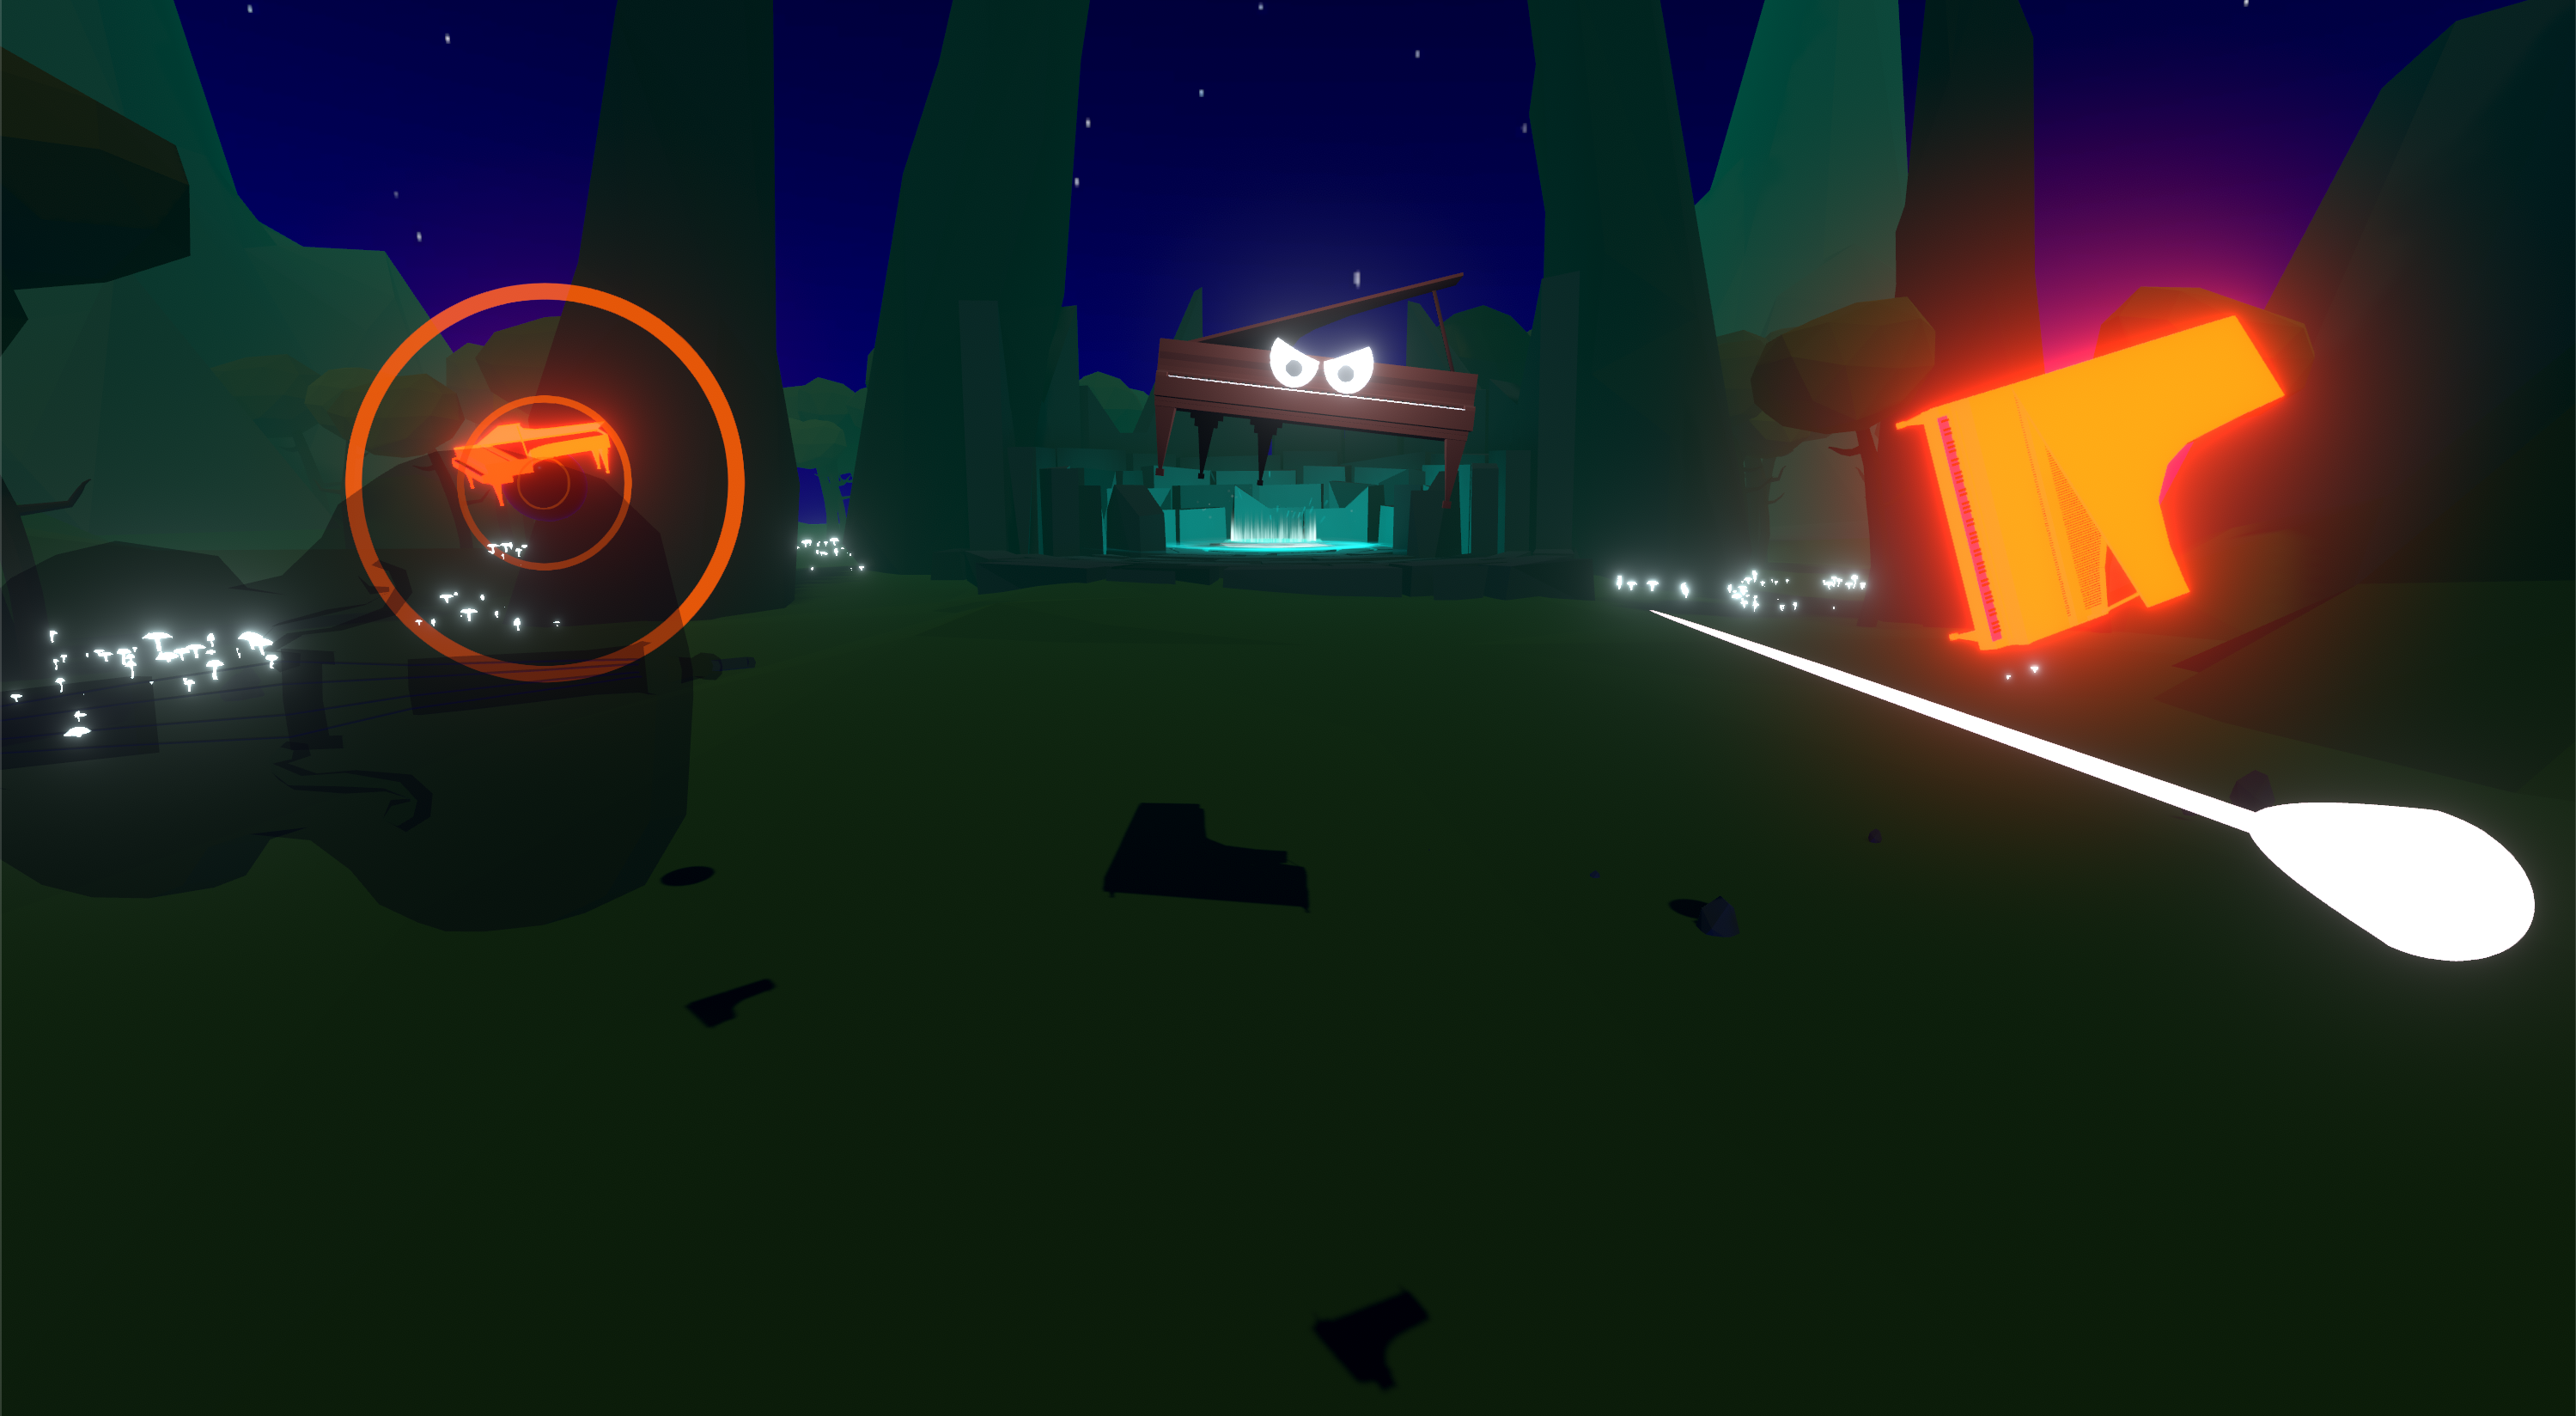
\includegraphics[width=0.75\textwidth]{figures/screenshots/harpsichord.png}
    \caption[The Harpsichord Distractor]{This screenshot shows the harpsichord distractor. It attacks with multiple rapid projectiles from two locations which are further away from its body.}
    \label{fig:harpsichordDistractor}
\end{figure}
''The Harpsichord'', which can be seen in Figure~\ref{fig:harpsichordDistractor} is the third distractor in Ensemble Retriever. It attacks the player with rapid projectiles that spawn from two wormholes that are further away from its body. This attack method means that the player needs to move their shield from left to right to quickly block incoming projectiles. It allows for some extra head rotation as the player might need to slightly shift their head to clearly see each projectile. 

\subsection{The Violin}
\begin{figure}[tbph]
    \centering
    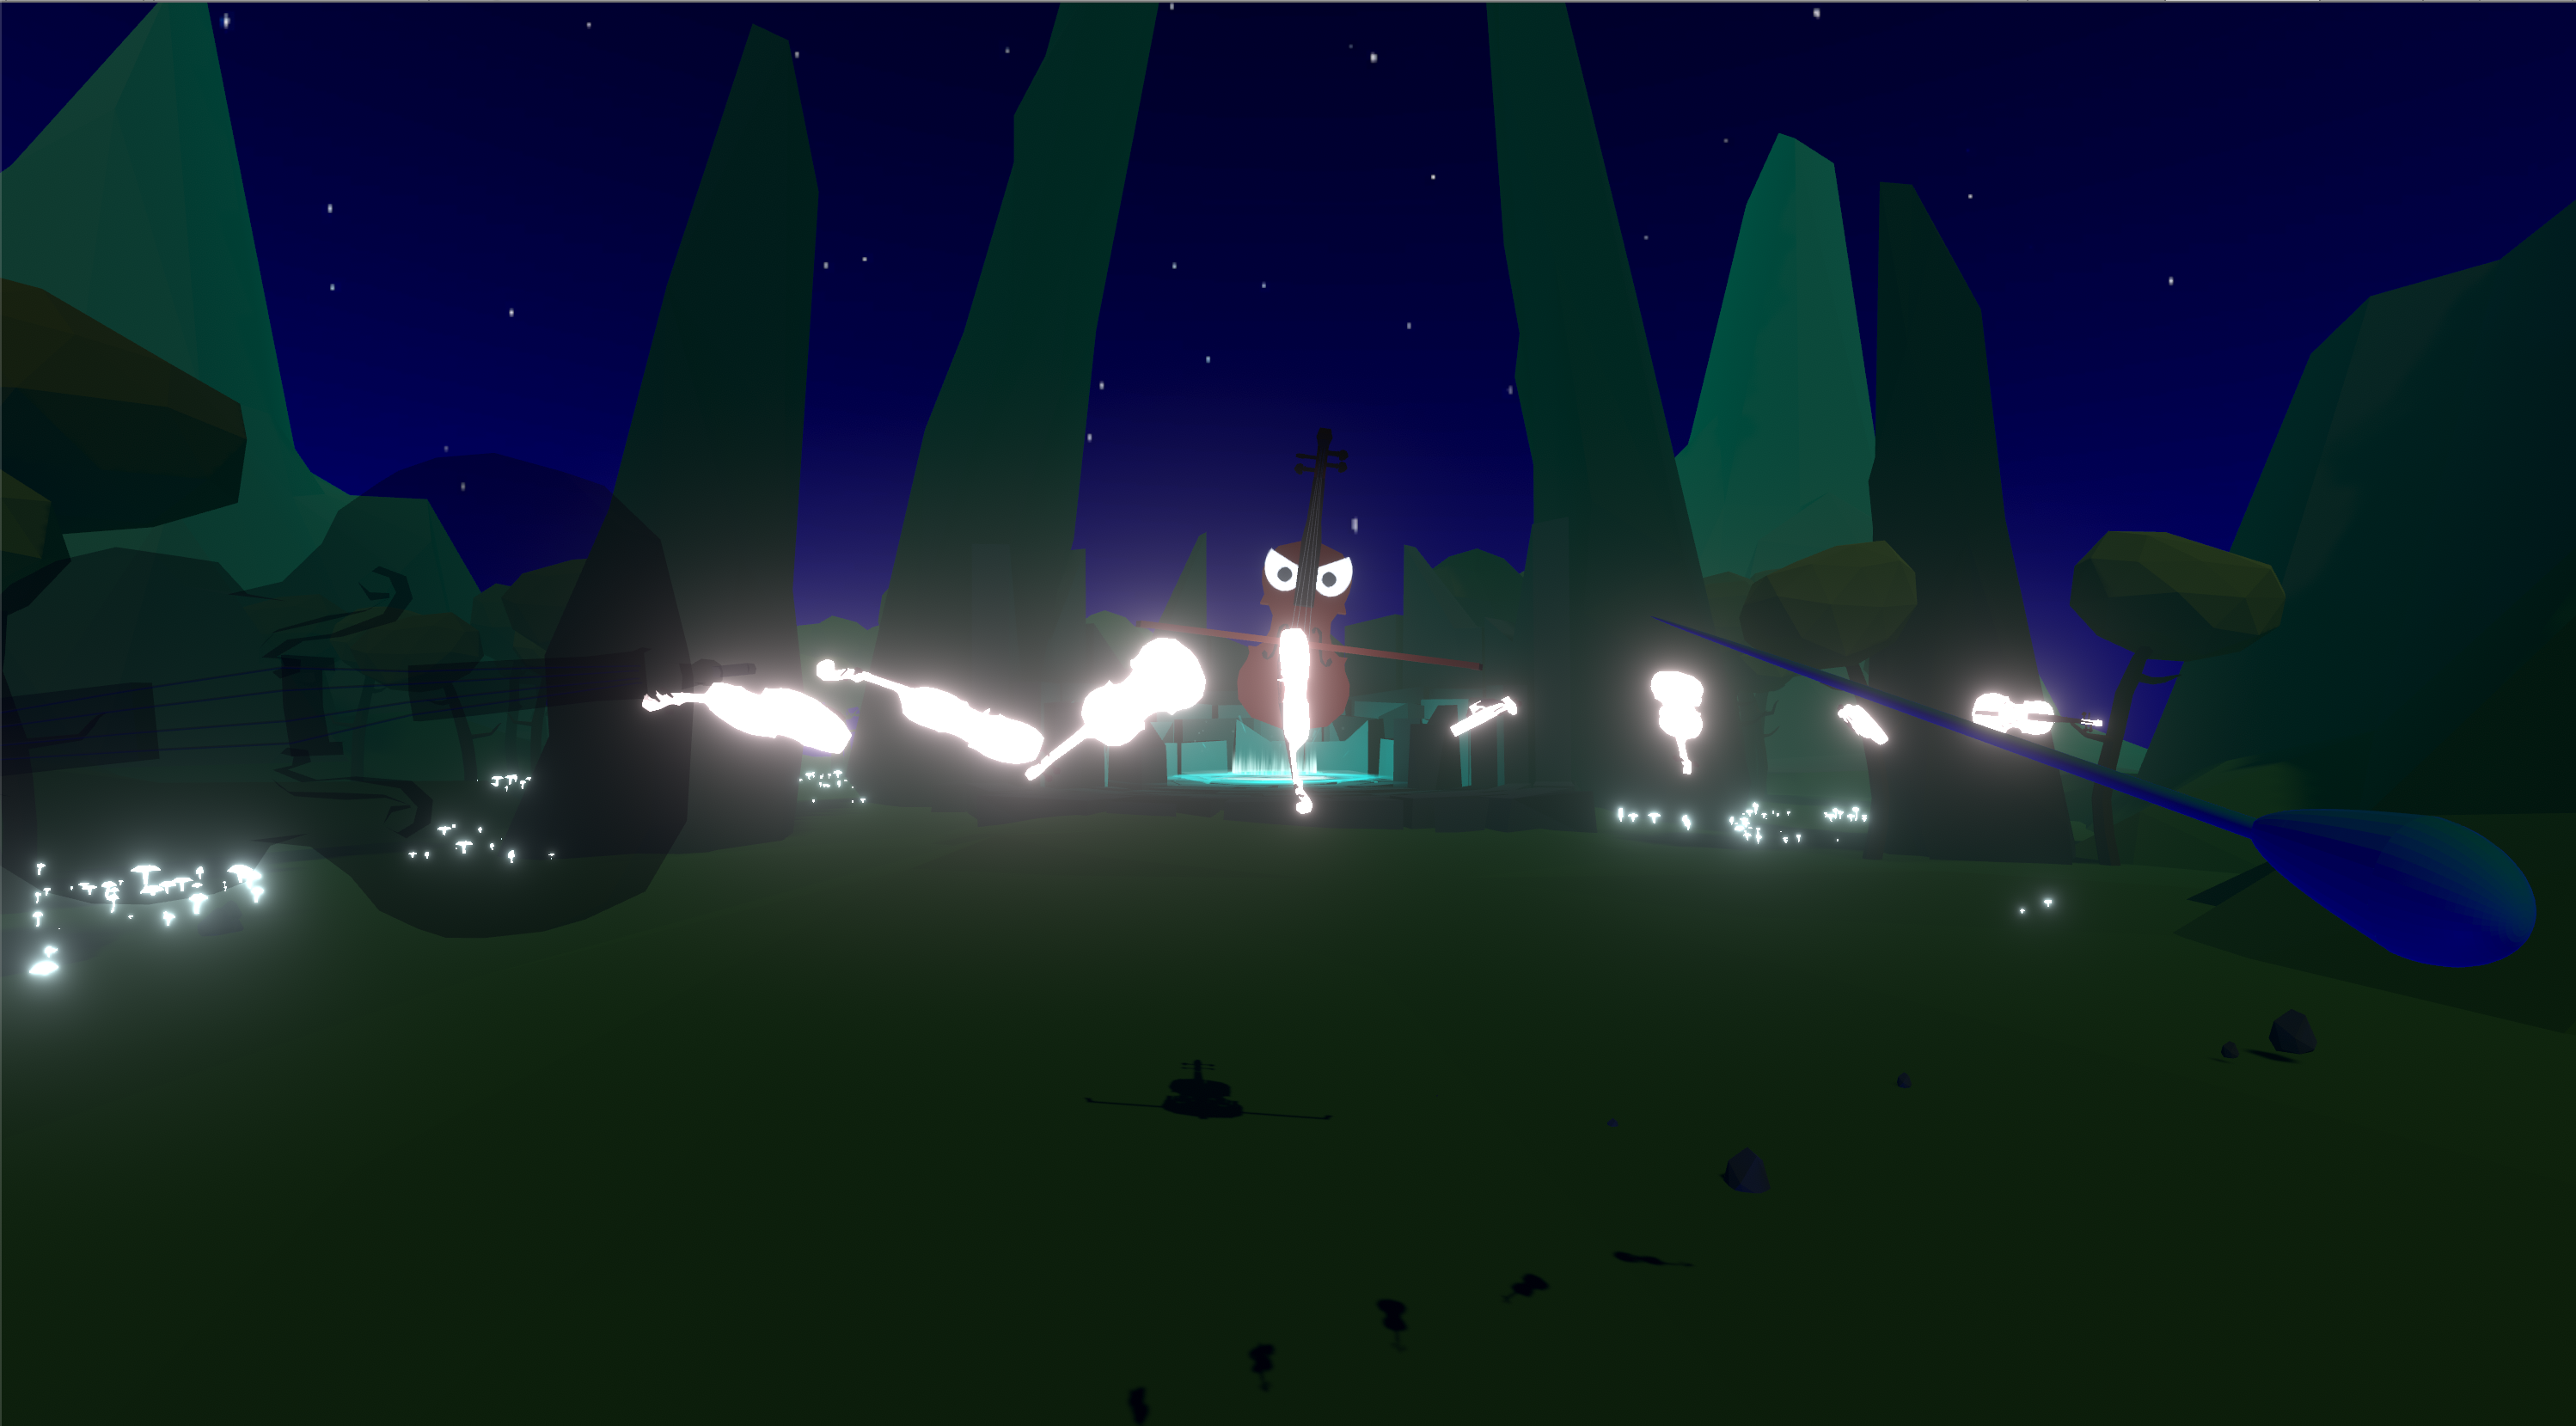
\includegraphics[width=0.75\textwidth]{figures/screenshots/violin.png}
    \caption[The Violin Distractor]{This screenshot shows the violin distractor. It attacks with several projectiles at a time in a line formation.}
    \label{fig:violinDistractor}
\end{figure}
The fourth distractor in Ensemble Retriever is ''The Violin'', which can be seen in Figure~\ref{fig:violinDistractor}. It is similar to the Harpsichord in the regard that it rapidly fires projectiles. Instead of firing projectiles from two locations though, it instead fires a line of projectiles that the player needs to block with their shield. This approach allows for some additional head rotation as the player needs to trace the line of projectiles that moves towards them. The line itself is long enough that some shifting of head orientation is beneficial to see everything as it gets close. 

\subsection{The Glockenspiel}
\begin{figure}[tbph]
    \centering
    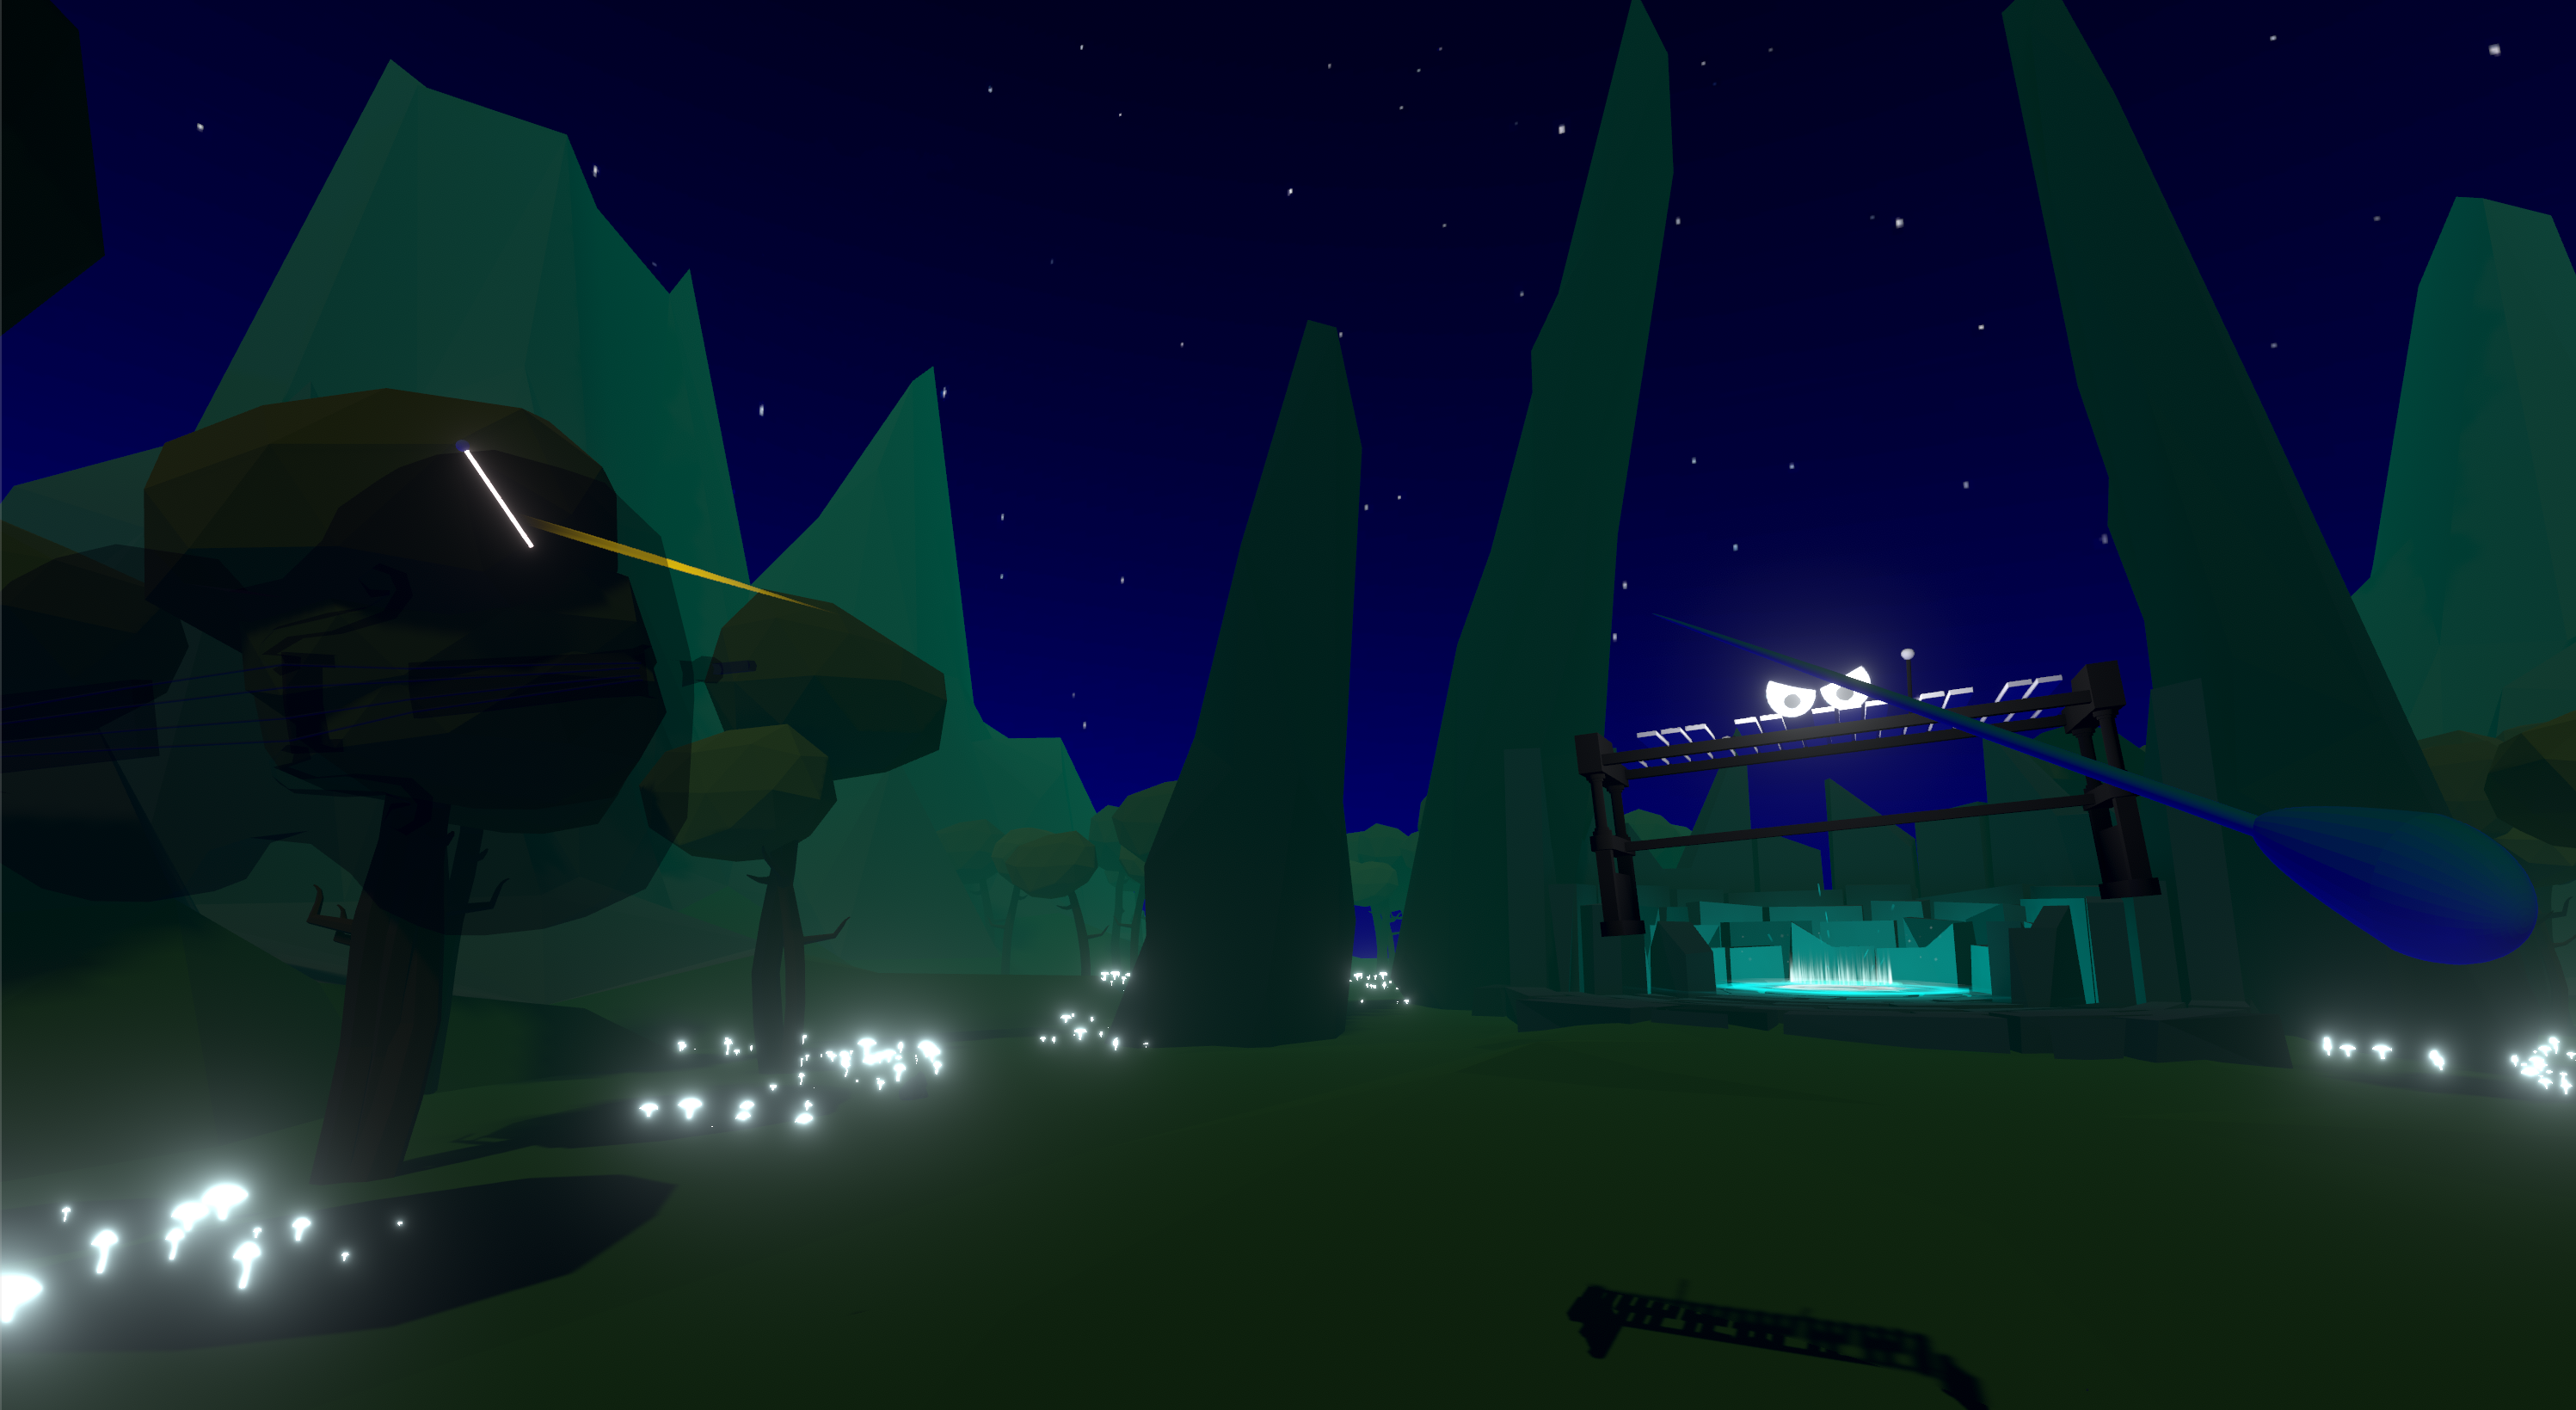
\includegraphics[width=0.75\textwidth]{figures/screenshots/glockenspiel.png}
    \caption[The Glockenspiel Distractor]{This screenshot shows the glockenspiel distractor and its curved projectile attack. The projectile itself travels on a arc towards the player's left side and will hit them at a \textasciitilde90 degree angle.}
    \label{fig:glockenspielDistractor}
\end{figure}
Finally, we have ''The Glockenspiel'', which is seen in Figure~\ref{fig:glockenspielDistractor}. This distractor attacks the player by throwing projectiles that travel on a curve towards the player. The curve itself will intersect with the player at a roughly 90-degree angle to their left from where the projectile was fired. This approach facilitates more head rotation as the player needs to track the path that the projectile flies through before blocking. 

\section{Employing Context Sensitive Reorientation: Teleporters}
While distractors are one example of context-sensitive reorientation, they are not necessarily the only ones that exist. There are many other potential options that can reorient the user while still being context sensitive. This thesis in particular makes use of one such method: reorientation when using teleporters. In games, when using a teleporter it is common to be reoriented in a manner so that they will face towards the future direction they are expected to walk. If we slightly modify this concept, we can make use of it for reorientation. As the player enters a portal or teleporter, their facing direction after being teleported is changed in a manner that results in their future expected path to be towards the room centre. As an example: in the Hall of The Mountain King, the player will be teleported to the edge of the room, meaning that there is only one direction they can walk in. By instantly reorienting the player during this teleportation it is possible to guarantee that this future direction will be through the centre of the physical space. 

In a way, this could be seen as similar to Suma et al.'s change blindness redirection~\cite{suma2011leveraging}, although it does not require the virtual world to dynamically change. The only thing that changes before and after teleportation in this case is the orientation of the user. Of course, this approach is not very useful if the teleporter sends the user to an open space as the future walking direction could vary. This reorientation method would most likely be at its most useful for more narrow spaces where potential walking directions are limited. In any case, it is a useful tool to consider as an alternative to only using distractors or other resetters. In the future, we may have many different types of context-sensitive reorientation methods outside of just distractors which all could exist together to create more varied experiences. For example, a cylindrical elevator which limits visibility could be used as a context-sensitive reorientation. In this case, it could reorient the user by having a door appear which forces the user to travel through the room centre when leaving. As Sra et al. already have discussed~\cite{sra2018vmotion}, anything that obscures or limits visibility in one way or another can be used to reorient or redirect a user. 


\section{Disabling Redirected Walking Towards the End of an Experience}
One particular detail that is further worth clarifying with Ensemble Retriever is that the redirection gains are disabled once the Hall of the Mountain King is entered. The reasoning behind this is so that participants can get used to normal head rotations before taking off their HMD and finishing the experience. Given that adaptation towards redirection is possible~\cite{bolling2019shrinking, grechkin2016revisiting}, it might be ideal to allow users to adapt back towards normal head rotation before they take off their HMD to limit any disorientation symptoms. How effective this approach is on the other hand, has not been measured and would need to be further tested in future work. Regardless, it is something that likely should be considered when developing redirected walking experience to ease the user back into how real head rotation functions. This approach might not necessarily be as easy to integrate with every solution, but it works well in the case of Ensemble Retriever. Since the final battle with the Mountain King occurs in a space where little movement is needed, there is also little need for redirection.

\section{Providing a Distance Magnitude Cooldown on Distractor Triggers}
One small detail that is worth to mention in Ensemble Retriever is the cooldown for triggering a new distractor after one has been defeated. A common way to handle this would be to have a timed cooldown. This would avoid immediately triggering a new distractor if the player is standing roughly on the bounds of the distractor trigger before starting to move again. If the player is standing still on this bounds for a longer amount of time though, this solution will not be effective. Instead, the player is required to walk a set amount of distance before a new distractor can trigger. This is not necessarily an ideal solution either as the maximum safe distance needed to travel before triggering a new distractor would vary depending on room size and require individual calibration. Furthermore, there are some additional issues which are mentioned in Section~\ref{sec:idealAlgorithmTimingSwitch}. The current implementation with a distance cooldown is the best solution which could be thought of for this thesis, but there are likely better alternatives which could be considered. 